\chapter{Expresiones Regulares y Análisis Léxico en JavaScript}
\label{chapter:expresionesregularesyanalisslexico}
%  Power Sh. JavaScript Cookbook. Chapter 1. Working with JavaScript Strings
%  David Flanagan. JavaScript, the Definitive Guide. O'Reilly.  Chapter 10.
%  JavaScript. The Missing Manual. Chapter 4. working with words, numbers and dates. A quick object lesson

\section{Mozilla Developer Network: Documentación}

\begin{enumerate}
\item \htmladdnormallink{RegExp Objects}{https://developer.mozilla.org/en-US/docs/JavaScript/Reference/Global_Objects/Regexp}
\item 
\htmladdnormallink{exec}{https://developer.mozilla.org/en-US/docs/JavaScript/Reference/Global_Objects/RegExp/exec}
\item 
\htmladdnormallink{search}{https://developer.mozilla.org/en-US/docs/JavaScript/Reference/Global_Objects/String/search}
\item 
\htmladdnormallink{match}{https://developer.mozilla.org/en-US/docs/JavaScript/Reference/Global_Objects/String/match}
\item 
\htmladdnormallink{replace}{https://developer.mozilla.org/en-US/docs/JavaScript/Reference/Global_Objects/String/replace}
\end{enumerate}

\sectionpractica{Conversor de Temperaturas}
\label{sectionpractica:conversordetemperaturas}

\parrafo{Donde}
\label{parrafo:dondetemperatura}
Véase 
\htmladdnormallink{https://bitbucket.org/casiano/pl-grado-temperature-converter/src}{https://bitbucket.org/casiano/pl-grado-temperature-converter/src}.
Este repo en bitbucket es privado del profesor.
El de 
\htmladdnormallink{GitHub }{https://github.com/crguezl/ull-etsii-grado-pl-1213-temperature-converter/tree/master}
es público pero no está completo.
\begin{verbatim}
~/local/src/javascript/PLgrado/temperature(master)]$ git remote -v
github  git@github.com:crguezl/ull-etsii-grado-pl-1213-temperature-converter.git (fetch)
github  git@github.com:crguezl/ull-etsii-grado-pl-1213-temperature-converter.git (push)
origin  ssh://git@bitbucket.org/casiano/pl-grado-temperature-converter.git (fetch)
origin  ssh://git@bitbucket.org/casiano/pl-grado-temperature-converter.git (push)
\end{verbatim}

Hay varias ramas (2015):

\begin{verbatim}
[~/local/src/javascript/PLgrado/temperature(master)]$ git branch -a
  gh-pages
  html5pattern
  karma
* master
  remotes/github/gh-pages
  remotes/github/master
  remotes/origin/html5pattern
  remotes/origin/karma
  remotes/origin/master
[~/local/src/javascript/PLgrado/temperature(master)]$
\end{verbatim}
\begin{itemize}
\item
En la rama \verb|master| está la versión mas simple.
\item
En la rama \verb|html5pattern| se muestra como usar el atributo \verb|pattern| (HTML5) 
en el tag \verb|input|.

En 29/09/2015 está disponible en el 
\htmladdnormallink{remoto github}{https://github.com/crguezl/ull-etsii-grado-pl-1213-temperature-converter/tree/html5pattern}.

Véase también
\htmladdnormallink{W3Schools}{http://www.w3schools.com/tags/att_input_pattern.asp}.
\item
Las pruebas están en el directorio \verb|tests/| en la rama master  que hay en GitHub 
\item
En la rama \verb|karma| (no visible al alumno, no está en GitHub en 2015) se encuentra como usar Karma para la ejecución de las pruebas.
En una práctica posterior se introduce Karma.
\end{itemize}


En mi portátil (29/09/2015) un clon del repo se encuentra en:
\begin{verbatim}
[~/srcPLgrado/temperature(master)]$ pwd -P
/Users/casiano/local/src/javascript/PLgrado/temperature # 27/01/2014
\end{verbatim}

\parrafo{index.html}

    \begin{verbatim}
<html>
  <head>
     <meta http-equiv="Content-Type" content="text/html; charset=UTF-8">
     <title>JavaScript Temperature Converter</title>
     <link href=normalize.css" rel="stylesheet" type="text/css">
     <link href="global.css" rel="stylesheet" type="text/css">

     <script type="text/javascript" src="temperature.js"></script>
  </head>
  <body>
    <h1>Temperature Converter</h1>
    <table>
      <tr>
        <th>Enter  Temperature (examples: 32F, 45C, -2.5f):</th>
        <td><input id="original" autofocus onchange="calculate();" placeholder="32F" size="50"></td>
      </tr>
      <tr>
        <th>Converted Temperature:</th>
        <td><span class="output" id="converted"></span></td>
      </tr>
    </table>
  </body>
</html>
    \end{verbatim}

\parrafo{Instale Emmet}

  Escribir HTML es farragoso. Una solución es usar algún plugin para su editor favorito.

Emmet existe para diversos editores, entre ellos para 
\begin{itemize}
\item
  En el caso de vim podemos usar 
\htmladdnormallink{Emmet-vim}{https://raw.githubusercontent.com/mattn/emmet-vim/master/TUTORIAL}
decargandolo desde 
\htmladdnormallink{http://www.vim.org/}{http://www.vim.org/scripts/script.php?script_id=2981}.

\item
Para \htmladdnormallink{Atom}{https://github.com/atom/atom}:
podemos usar
\htmladdnormallink{Plugin Emmet para Atom en GitHub}{https://github.com/emmetio/emmet-atom}
\begin{itemize}
\item
\htmladdnormallink{cheat-sheet}{http://sweetme.at/2014/03/10/atom-editor-cheat-sheet/} de Atom
\item
Véase el artículo \htmladdnormallink{Recommended GitHub Atom Packages for Web Developers}{http://www.elijahmanor.com/github-atom-packages/}.
\end{itemize}
\item
En
cloud9 
(\htmladdnormallink{c9.io}{https://c9.io/})
el plugin ya viene instalado
\end{itemize}

\begin{itemize}
\item
\htmladdnormallink{Documentación de Emmet}{http://docs.emmet.io/}
\item
\htmladdnormallink{Emmet cheat sheet}{http://docs.emmet.io/cheat-sheet/}
\end{itemize}

\parrafo{input tag}
\begin{itemize}
\item
The 
\htmladdnormallink{input}{http://www.w3schools.com/tags/tag_input.asp}
tag specifies an input field where the user can enter data.

\item
\verb|<input>| elements are used within a \verb|<form>| element to declare input controls that allow users to input data.

\item
An input field can vary in many ways, depending on the \verb|type| attribute.

\item
The \verb|type| attribute specifies the type of \verb|<input>| element to display.
The default type is \verb|text|.

Other values are:
\begin{itemize}
\item button
\item checkbox
\item color
\item date 
\item datetime 
\item datetime-local 
\item email 
\item file
\item hidden
\item image
\item month 
\item number 
\item password
\item radio
\item range 
\item reset
\item search
\item submit
\item tel
\item text
\item time 
\item url
\item week
\end{itemize}
\item
The elements used to create controls generally appear inside a \verb|<form>| 
element, but may also appear outside of a \verb|<form>| element declaration.
\end{itemize}

\parrafo{onchange}
The \verb|onchange| event occurs when the value of an element has been changed.

\parrafo{link tag}
\begin{itemize}
\item
The \verb|<link>| tag defines a link between a document and an external resource.
\begin{verbatim}
     <link href="global.css" rel="stylesheet" type="text/css">
\end{verbatim}
\item
The \verb|rel| attribute is required. It specifies the relationship between the current document and the linked document
\item
The \verb|<link>| tag is used to link to external CSS style sheets.
\begin{verbatim}
 <link href="global.css" rel="stylesheet" type="text/css">
\end{verbatim}
\end{itemize}

\parrafo{CSS}

\cei{CSS} stands for \cei{Cascading Style Sheets} and is a separate, but complementary, language to HTML. CSS is what we use to apply styles to the content on our web page.

\parrafo{global.css}


    \begin{verbatim}
[~/srcPLgrado/temperature(master)]$ cat global.css 
th, td      { vertical-align: top; text-align: right; font-size:large; }     /* Don't center table cells  */
#converted  { color: red; font-weight: bold; font-size:large;          }     /* Calculated values in bold */
input       { 
              text-align: right;       /* Align input to the right  */
              border: none; 
              border-radius: 20px 20px 20px 20px;
              padding: 5px  5px;
              font-size:large;       }
body
{
 background-color:#b0c4de;  /* blue */
 font-size:large;
 font-family: "Lucida Sans Typewriter", "Lucida Console", Monaco, "Bitstream Vera Sans Mono", monospace;
}

h1 {
    font-weight: normal;
    font-family: "Brush Script MT", cursive;
    background: #3C5681;
    padding: 5px 15px;
    color: white;
    display:inline-block;
    border-radius: 10px 10px 10px 10px;
}
    \end{verbatim}
  
\parrafo{Sintáxis CSS}

\begin{verbatim}
th, td      { vertical-align: top; text-align: right; font-size:large; }     /* Don't center table cells  */
\end{verbatim}
What you see above is referred to as a \cei{rule set}. 

\begin{itemize}
\item
Notice the curly braces. Also, notice that each declaration inside the curly braces has a semicolon. Everything
inside the curly braces is called a \cei{declaration block}.
\item
The portion prior to the first curly brace is what defines which part of the web page we are styling. This is referred to as the \cei{selector}.

Here we're using commas to separate our selectors \verb|th| and \verb|td|. 
This is a useful method to use to combine multiple selectors in a single rule set. 
In this case, the styles will apply to all \verb|<th>| and \verb|<td>| elements,
\item
Each of the three declarations in the declaration block is referred to as a \cei{declaration}. 
\item
Additionally, each declaration consists of a \cei{property} (the part before the colon)
and a \cei{value} (the part after the colon). 
\item
Each CSS declaration ends with a semicolon.
\end{itemize}

\parrafo{Introducción a los Selectores CSS}
\begin{itemize}
\item
A selector of \verb|nav| would match all HTML \verb|<nav>| elements, and a selector of \verb|ul| would match all HTML unordered lists, or \verb|<ul>| elements.
\item
An ID selector is declared using a hash, or pound symbol (\verb|#|) 
preceding a string of characters. 
The string of characters is defined by the developer. 
This selector matches any HTML element that has an
\verb1ID1 attribute with the same value as that of the selector, but minus the hash symbol.

The rule:
\begin{verbatim}
#converted  { color: red; font-weight: bold; font-size:large; } /* Calculated values in bold */
\end{verbatim}
applies to:
\begin{verbatim}
<span class="output" id="converted">
\end{verbatim}
\item
An ID element on a web page should be unique. 
\end{itemize}

\begin{exercise}
Usa 
\htmladdnormallink{jsfiddle.net}{https://jsfiddle.net}
para encontrar las respuestas a las preguntas. 
\begin{itemize}
\item \cei{Descendant Selector}:

Dado el selector
\begin{verbatim}
#container .box {
   float: left;
   padding-bottom: 15px;
}
\end{verbatim}
¿A que elementos de este HTML se aplica?
\begin{verbatim}
<div id="container">
  <div class="box"></div>
  <div class="box-2"></div>
</div>

<div class="box"></div>
\end{verbatim}
This declaration block will apply to all elements that have a class of box that are inside an element with an \verb|ID| of container. It's worth noting that the \verb|.box|
element doesn't have to be an immediate
child: there could be another element wrapping \verb|.box|, 
and the styles would still apply.
\item \cei{Child selector} (targets immediate child elements):

Dada esta regla
\begin{verbatim}
#container > .box {
   float: left;
   padding-bottom: 15px;
}
\end{verbatim}
In this example, the selector will match all elements that have a class of 
\verb|box| and that are immediate children of the 
\verb|#container| element. 
That means, unlike the descendant combinator, there can't be
another element wrapping \verb|.box|: 
it has to be a direct child element.


¿A que elementos de este HTML se aplica?
\begin{verbatim}
<div id="container">
  <div class="box"></div>
  <div>
    <div class="box"></div>
  </div>
</div>
\end{verbatim}

In this example, the CSS from the previous code example will apply only to the first 
\verb|<div>| element that has a class of \verb|box|. 

As you can see, the second \verb|<div>|
element with a class of box is inside
another \verb|<div>| element. 
As a result, the styles will not apply to that element, even though it too has a class of 
\verb|box|.

\item A general \cei{sibling combinator} matches elements based on sibling (hermanos)
relationships. That is to say, the selected elements are beside each other in the HTML.

Dada esta regla % hermanos: a los <p> que son hermanos de h2
\begin{verbatim}
h2 ~ p { margin-bottom: 20px; }
\end{verbatim}

This type of selector is declared using the tilde character (\verb|~|). 
In this example, all paragraph elements (\verb|<p>|) 
will be styled with the specified rules, but only if they are siblings of 
\verb|<h2>| elements.
There could be other elements in between the \verb|<h2>| and 
\verb|<p>|, and the styles would still apply.

¿A que elementos de este HTML se aplica?
\begin{verbatim}
<h2>Title</h2>
<p>Paragraph example 1.</p>
<p>Paragraph example 2.</p>
<p>Paragraph example 3.</p>
<div class="box">
  <p>Paragraph example 4.</p>
</div>
\end{verbatim}
\item 
The \cei{adjacent sibling combinator} uses the plus symbol (\verb|+|), 
and is almost the same as the general sibling selector. 
The difference is that the targeted element must be an immediate sibling, not just a general sibling. 

Dada esta regla 
% hermanos adyacentes: a los p que son hermanos adyacentes de un p
\begin{verbatim}
p+ p {
text-indent: 1.5em; margin-bottom: 0;
}
\end{verbatim}
This example will apply the specified styles
only to paragraph elements that immediately follow other paragraph elements.
the first paragraph element on a page would not receive these styles.
Also, if another element appeared between two paragraphs, the second paragraph of the two wouldn't have the styles applied.

¿A que elementos de este HTML se aplica?
\begin{verbatim}
<h2>Title</h2>
<p>Paragraph example 1.</p>
<p>Paragraph example 2.</p>
<p>Paragraph example 3.</p>
<div class="box">
  <p>Paragraph example 4.</p>
  <p>Paragraph example 5.</p>
</div>
\end{verbatim}
% ...the styles will apply only to the second, third, and fifth paragraphs in this section of HTML.
\item The \cei{attribute selector} 
targets elements based on the presence and/or value of HTML attributes, and is declared using square brackets.

There should not be a space before the opening square bracket unless you intend to use it along with a {\it descendant combinator}. 


Dada esta regla:
\begin{verbatim}
input[type="text"] {
   background-color: #444;
   width: 200px;
}
\end{verbatim}
The attribute selector targets elements based on the presence and/or value of HTML attributes, and is declared using square brackets.

¿A que elementos de este HTML se aplica?
\begin{verbatim}
  <input type="text">
  <input type="submit">
\end{verbatim}
\item A \cei{pseudo-class} 
uses a colon character to identify a pseudo-state that an element might be in.


Dada esta regla:
\begin{verbatim}
a:hover {
   color: red;
}
\end{verbatim}
¿Que porción del selector es conocido como \cei{pseudo-clase}?
¿Cuando se aplica la regla a un ancla \verb|<a>|?

In this case, the pseudo-class portion of the selector is the \verb|:hover| part. 
Here we've attached this pseudo-class to all anchor elements 
(\verb|<a>| elements). 
This means that when the user hovers their mouse
over an \verb|<a>| element, the color property for that element will change to red. 

This type of pseudo-class is a \cei{dynamic pseudo-class}, 
because it occurs only in response to user interaction—in this case,
the mouse moving over the targeted element.

It's important to recognize that these types of selectors do not just select elements; 
\emph{they select elements that are in a particular state}. 

% It's important to recognize that these types of selectors do not just select elements; they select elements that are in a particular state
\item 

Exprese con palabras a que elementos del documento se aplicará la siguiente regla:
\begin{verbatim}
#form [type=text] { border: solid 1px #ccc; }
\end{verbatim}

This selector combines the \verb|ID| selector with the attribute selector. 

This will target all elements with a type attribute of \verb|text| that are inside an element with an \verb|ID| of 
\verb|form|.

\end{itemize}
\end{exercise}

\begin{exercise}
\begin{itemize}
\item
Supuesto que una hoja de estilo contiene estas reglas:
\begin{verbatim}
p { font-size: 20px; }
p { font-size: 30px; } 
\end{verbatim}
¿Cual será el tamaño de font que se aplique a los elementos párrafo?

\red{Selectors targeting styles later in a CSS document have precedence over the same selectors that appear earlier in the CSS file}. 
\item
Supuesto que una hoja de estilo contiene estas reglas:
\begin{verbatim}
div p { color: blue; }
p{ color: red; }
\end{verbatim}
¿Cual será el color que se aplique a los elementos párrafo?
% the descendant selector takes precedence over the element type selector

In this instance, the color value for paragraph elements inside of \verb|<div>|
elements will be blue, despite the fact that the second color declaration
appears later in the document. \red{So although the browser
does give some importance to the order of these rule sets, that order
is superseded by the} {\bf specificity} of the first rule set.
\item
Supuesto que una hoja de estilo contiene estas reglas:
\begin{verbatim}
#main {
   color: green;
}
body div.container {
   color: pink;
}
\end{verbatim}
¿Cual será el color que se aplique a este elemento \verb|<div>|?
\begin{verbatim}
<div id="main" class="container"></div>
\end{verbatim}


\red{The ID selector has very high specificity}
and thus takes precedence over the second rule set.
\end{itemize}
\end{exercise}

\parrafo{CSS reset}
Every browser applies certain styles to elements on a web page by default. 

For example, if you use an un-ordered list (the \verb|<ul>| element) the browser will display the list with some existing
formatting styles, including bullets next to the individual list items (the \verb|<li>| elements inside the \verb|<ul>|). 

By using a \cei{CSS reset document} at the top of your CSS file, you can reset all these styles
to a bare minimum. 


Two of the most popular CSS resets are 
\htmladdnormallink{Eric Meyer's Reset }{http://meyerweb.com/eric/tools/css/reset/}
and 
\htmladdnormallink{Nicolas Gallagher's Normalize.css}{http://necolas.github.io/normalize.css/}

\begin{verbatim}
    <title>JavaScript Temperature Converter</title>
    <link href=normalize.css" rel="stylesheet" type="text/css">
    <link href="global.css" rel="stylesheet" type="text/css">
\end{verbatim}

\parrafo{El Modelo de Caja}

The \cei{box model} refers to the usually invisible rectangular area that is created for each HTML element. This area has four basic components

\begin{rawhtml}
<img src="cssboxmodel.png" align="middle" />
\end{rawhtml}


\begin{itemize}
\item
\cei{Content} 

The content portion of the box model holds the actual content. 

The content can be text, images, or
whatever else is visible on a web page.

\item
\cei{Padding}

The \verb|padding| of an element is defined using the \verb|padding| property. The \verb|padding| is the space around the content. 

It can be defined for an individual side 
(for example, \verb|padding-left: 20px|) or
for all four sides in one declaration
\verb|padding: 20px 10px 30px 20px|, for instance. 

When declaring all four sides, you’re using a \cei{shorthand property}. 

Often when a CSS property takes multiple values like this, \blue{they start at the top and go clockwise in relation to the element}. 
So, in the example just cited, this would apply \verb|20px| of padding to the
top, \verb|10px| to the right, \verb|30px| to the bottom, and \verb|20px| to the left.

  See \htmladdnormallink{padding examples at w3schools}{http://www.w3schools.com/css/css_padding.asp}.
\item
\cei{Border} 

The border of an element is defined using the border property. 

This is a \red{shorthand property} that defines the element's \verb|border-width|, \verb|border-style|, and \verb|border-color|. For example, 
\begin{verbatim}
border: 4px dashed orange.
\end{verbatim}

\item
\cei{Margin} 

Margins are similar to padding, and are defined using similar syntax 

\begin{verbatim}
margin-left: 15px
\end{verbatim}
or
\begin{verbatim}
 margin: 10px 20px 10px 20px
\end{verbatim}
The margin portion of an element exists outside the element. 

\blue{A margin creates space between the targeted element and surrounding elements}.
\end{itemize}

\begin{exercise}
\begin{itemize}
\item Dadas las declaraciones:
\begin{verbatim}
.example {
  border-style: dashed;
  border-width: 2px;
  border-color: blue;
}
.example {
  border: solid;
  color: green;
}
\end{verbatim}
¿De que color queda el borde de los elementos de clase \verb|example|? 
¿Que \verb|border-style| tendrán?
¿Que \verb|border-width| tendrán?

Here we’ve used the same selector on two different rule sets. 

The second rule set will take precedence over the first, overriding any styles that are the same in both rule sets.

In the first rule set, we’ve defined all three \verb|border-related| properties in longhand, setting the values to display a dashed border that’s 2px wide and colored blue. 

But what’s the result of these two
rule sets? Well, the border will become 3px wide 
(the default border width for a visible border,) and it'll be colored green, not blue. 

This happens because the second rule set uses shorthand to
define the \verb|border-style| as solid, \emph{but doesn’t define the other two properties} (\verb|border-width| and 
\verb|border-color|).

See
\begin{itemize}
\item
\htmladdnormallink{jsfiddle}{https://jsfiddle.net/casiano/u3nrjssa/}
\item
\htmladdnormallink{gist}{https://gist.github.com/crguezl/40c6b3fd6b95cc3d5f97}
\end{itemize}

\item Dada la declaración:
\begin{verbatim}
.example {
  margin: 10px 20px;
}
\end{verbatim}
¿De que tamaño quedarán \verb|margin-top| \verb|margin-right|, \verb|margin-bottom| y \verb|margin-left| para los elementos de clase \verb|example|?

Another thing to understand about shorthand is that for certain shorthand properties, the missing values are inherited based on the existing values.

We’re omitting the bottom and left, so they'll inherit from the top and right values.

\end{itemize}
\end{exercise}

\parrafo{Editing CSS styles in Chrome using various DevTools aid}

Depurar estilos puede ser complicado. Lea el artículo
\htmladdnormallink{Tips for Debugging HTML and CSS}{http://blog.teamtreehouse.com/tips-debugging-html-css}.

While you can not "debug" CSS, because it is not a scripting language,
you can utilize the Chrome DevTools Elements panel to inspect an element and
view the Styles pane on the right. 

This will give you
insights as to the styles being overridden or ignored (line threw). 

The Styles pane is also useful because of it's ability to LiveEdit the document being inspected, which may help you iron out the
issues. 

If the styles are being overridden, you can then view the Computed Style pane to see the CSS that is actually being utilized to style your document.

\begin{itemize}
\item
\htmladdnormallink{Editing styles}{https://developer.chrome.com/devtools/docs/elements-styles}
in Chrome developer pages.
\item
\htmladdnormallink{stackoverflow: Debugging CSS in Google Chrome}{http://stackoverflow.com/questions/11065229/debugging-css-in-google-chrome}
\item
\htmladdnormallink{Chrome DevTools for CSS - Better CSS Coding and CSS Debugging with Developer Tools}{http://youtu.be/Z3HGJsNLQ1E} en YouTube by LearnCode.academy
\end{itemize}

\parrafo{Block versus Inline}

HTML elements fall under two categories: \cei{block} or \cei{inline}.


\begin{itemize}
\item
Block-level elements include elements like \verb|<div>|, \verb|<p>|, \verb|h1|, \verb|li|
and \verb|<section>|.
A block-level element is more of a structural, layout related element.

\red{A block element is an element that takes up the full width available, and has a line break before and after it}.
\item
\blue{An inline element only takes up as much width as necessary, and does not force line breaks}.
Inline elements behave like words and letters within of a paragraph.

Inline elements include \verb|<span>|, \verb|<b>|, and \verb|<em>|.

It's worth noting that inline elements are subject to CSS properties that affect text. 

For example, \verb|line-height| and \verb|letter-spacing| are CSS properties that can be used to style inline elements.

However, those same properties wouldn't affect block elements.

\item
See 
\begin{itemize}
\item
\htmladdnormallink{CSS display Property}{http://www.w3schools.com/cssref/pr_class_display.asp}
\item
\htmladdnormallink{CSS Display - Block and Inline Elements at w3schools}{http://www.w3schools.com/css/css_display_visibility.asp}
\end{itemize}
\end{itemize}

\parrafo{Propiedades CSS}
\begin{itemize}
\item
The 
\htmladdnormallink{vertical-align}{http://www.w3schools.com/cssref/pr_pos_vertical-align.asp}
property sets the vertical alignment of an element.
\item
The 
\htmladdnormallink{text-align}{http://www.w3schools.com/cssref/pr_text_text-align.asp}
property specifies the horizontal alignment of text in an element.
\item
The 
\htmladdnormallink{font-family}{http://www.w3schools.com/cssref/pr_font_font-family.asp}
property specifies the font for an element.

The font-family property can hold several font names as a "fallback" system. 
If the browser does not support the first font, it tries the next font.
\end{itemize}

\parrafo{temperature.js}


  \begin{latexonly}
    \begin{verbatim}

"use strict"; // Use ECMAScript 5 strict mode in browsers that support it
function calculate() {
  var result;
  var original       = document.getElementById("........");
  var temp = original.value;
  var regexp = /.............................../;
  
  var m = temp.match(......);
  
  if (m) {
    var num = ....;
    var type = ....;
    num = parseFloat(num);
    if (type == 'c' || type == 'C') {
      result = (num * 9/5)+32;
      result = ..............................
    }
    else {
      result = (num - 32)*5/9;
      result = ............................
    }
    converted.innerHTML = result;
  }
  else {
    converted.innerHTML = "ERROR! Try something like '-4.2C' instead";
  }
}

    \end{verbatim}
  \end{latexonly}
    \begin{rawhtml}
    <pre>
<span class="s2">&quot;use strict&quot;</span><span class="p">;</span> <span class="c1">// Use ECMAScript 5 strict mode in browsers that support it</span>
<span class="kd">function</span> <span class="nx">calculate</span><span class="p">()</span> <span class="p">{</span>
  <span class="kd">var</span> <span class="nx">result</span><span class="p">;</span>
  <span class="kd">var</span> <span class="nx">original</span>       <span class="o">=</span> <span class="nb">document</span><span class="p">.</span><span class="nx">getElementById</span><span class="p">(</span><span class="s2">&quot;........&quot;</span><span class="p">);</span>
  <span class="kd">var</span> <span class="nx">temp</span> <span class="o">=</span> <span class="nx">original</span><span class="p">.</span><span class="nx">value</span><span class="p">;</span>
  <span class="kd">var</span> <span class="nx">regexp</span> <span class="o">=</span> <span class="sr">/.............................../</span><span class="p">;</span>
  
  <span class="kd">var</span> <span class="nx">m</span> <span class="o">=</span> <span class="nx">temp</span><span class="p">.</span><span class="nx">match</span><span class="p">(......);</span>
  
  <span class="k">if</span> <span class="p">(</span><span class="nx">m</span><span class="p">)</span> <span class="p">{</span>
    <span class="kd">var</span> <span class="nx">num</span> <span class="o">=</span> <span class="p">....;</span>
    <span class="kd">var</span> <span class="nx">type</span> <span class="o">=</span> <span class="p">....;</span>
    <span class="nx">num</span> <span class="o">=</span> <span class="nb">parseFloat</span><span class="p">(</span><span class="nx">num</span><span class="p">);</span>
    <span class="k">if</span> <span class="p">(</span><span class="nx">type</span> <span class="o">==</span> <span class="s1">&#39;c&#39;</span> <span class="o">||</span> <span class="nx">type</span> <span class="o">==</span> <span class="s1">&#39;C&#39;</span><span class="p">)</span> <span class="p">{</span>
      <span class="nx">result</span> <span class="o">=</span> <span class="p">(</span><span class="nx">num</span> <span class="o">*</span> <span class="mi">9</span><span class="o">/</span><span class="mi">5</span><span class="p">)</span><span class="o">+</span><span class="mi">32</span><span class="p">;</span>
      <span class="nx">result</span> <span class="o">=</span> <span class="p">..............................</span>
    <span class="p">}</span>
    <span class="k">else</span> <span class="p">{</span>
      <span class="nx">result</span> <span class="o">=</span> <span class="p">(</span><span class="nx">num</span> <span class="o">-</span> <span class="mi">32</span><span class="p">)</span><span class="o">*</span><span class="mi">5</span><span class="o">/</span><span class="mi">9</span><span class="p">;</span>
      <span class="nx">result</span> <span class="o">=</span> <span class="p">............................</span>
    <span class="p">}</span>
    <span class="nx">converted</span><span class="p">.</span><span class="nx">innerHTML</span> <span class="o">=</span> <span class="nx">result</span><span class="p">;</span>
  <span class="p">}</span>
  <span class="k">else</span> <span class="p">{</span>
    <span class="nx">converted</span><span class="p">.</span><span class="nx">innerHTML</span> <span class="o">=</span> <span class="s2">&quot;ERROR! Try something like &#39;-4.2C&#39; instead&quot;</span><span class="p">;</span>
  <span class="p">}</span>
<span class="p">}</span>
    </pre>
    \end{rawhtml}
  
\parrafo{Despliegue}
\begin{itemize}
\item
Deberá desplegar la aplicación en GitHub Pages como página de proyecto.
Vea la sección {\it GitHub Project Pages} \ref{subsection:githubprojectpages}.
\end{itemize}

\parrafo{Creando un fichero package.json}

Para saber todo sobre 
\htmladdnormallink{ipackage.json}{https://docs.npmjs.com/files/package.json}
visite este manual de npm o bien escriba \verb|npm help json| en la línea de comandos.

The command:

\begin{verbatim}
npm init [-f|--force|-y|--yes]
\end{verbatim}

Will ask you a bunch of questions, and then write a \verb|package.json| for you.

If you already have a \verb|package.json| file, it'll read that first, and default to the options in there.

It is strictly additive, so it does not delete options from your \verb|package.json|
without a really good reason to do so.

If you invoke it with \verb|-f|, \verb|--force|, it will use only defaults and not prompt you for any options.

\begin{verbatim}
[/tmp/pl-grado-temperature-converter(karma)]$ npm init
This utility will walk you through creating a package.json file.
It only covers the most common items, and tries to guess sane defaults.

See `npm help json` for definitive documentation on these fields
and exactly what they do.

Use `npm install <pkg> --save` afterwards to install a package and
save it as a dependency in the package.json file.

Press ^C at any time to quit.
name: (pl-grado-temperature-converter) 
version: (0.0.0) 0.0.1
description: ULL ESIT Grado de Informática. 3º. PL. Lab "Temperature Converter"
entry point: (temperature.js) 
test command: open tests/index.html
git repository: (ssh://git@bitbucket.org/casiano/pl-grado-temperature-converter.git) 
keywords: regexp
author: Casiano
license: (ISC) 
About to write to /private/tmp/pl-grado-temperature-converter/package.json:

{
  "name": "pl-grado-temperature-converter",
  "version": "0.0.1",
  "description": "ULL ESIT Grado de Informática. 3º. PL. Lab \"Temperature Converter\"",
  "main": "temperature.js",
  "directories": {
    "test": "tests"
  },
  "scripts": {
    "test": "open tests/index.html"
  },
  "repository": {
    "type": "git",
    "url": "ssh://git@bitbucket.org/casiano/pl-grado-temperature-converter.git"
  },
  "keywords": [
    "regexp"
  ],
  "author": "Casiano",
  "license": "ISC"
}


Is this ok? (yes) y
\end{verbatim}

Esto genera el fichero \verb|package.json|:
\begin{verbatim}
[/tmp/pl-grado-temperature-converter(karma)]$ ls -ltr | tail -1
-rw-r--r--  1 casiano  wheel   487  5 feb 18:22 package.json
\end{verbatim}
Si ahora escribo:
\begin{verbatim}
[/tmp/pl-grado-temperature-converter(karma)]$ npm test

> pl-grado-temperature-converter@0.0.1 test /private/tmp/pl-grado-temperature-converter
> open tests/index.html
\end{verbatim}
Ejecutamos las pruebas en el navegador (en Mac OS X) supuesto que ya estuvieran escritas.




%\parrafo{Pruebas: Mocha y Chai}
\parrafo{Pruebas: Mocha y Chai}
\label{parrafo:mochaychai}
Mocha is a test framework while Chai is an expectation one. 

Mocha is the \red{simple, flexible, and fun} JavaScript unit-testing framework
that runs in Node.js or in the browser. 

It is open source (MIT licensed),
and we can learn more about it at
\htmladdnormallink{https://github.com/mochajs/mocha}{https://github.com/mochajs/mocha}

Let's say
Mocha setups and describes test suites and Chai provides convenient
helpers to perform all kinds of assertions against your JavaScript code.

\parrafo{Pruebas: Estructura}

Podemos instalar \verb|mocha| globalmente:
\begin{verbatim}
$ npm install -g mocha
\end{verbatim}
pero podemos también añadirlo en \verb|package.json| como una \verb|devDependencies|:
\begin{verbatim}
[/tmp/pl-grado-temperature-converter(karma)]$ head -n 5 package.json 
{
  "dependencies": {},
  "devDependencies": {
    "mocha": "latest"
  },
\end{verbatim}

Y ahora podemos instalar todas las dependencias usando  \verb|npm install|:
\begin{verbatim}
$ npm install
npm http GET https://registry.npmjs.org/mocha
npm http 200 https://registry.npmjs.org/mocha
npm http GET https://registry.npmjs.org/commander/2.3.0
...
\end{verbatim}

En este caso \verb|mocha| es instalado localmente, no globalmente:
\begin{verbatim}
[/tmp/pl-grado-temperature-converter(karma)]$ ls -ltr node_modules/
total 0
drwxr-xr-x  12 casiano  staff  408  5 feb 18:40 mocha
\end{verbatim}

Una vez instalado Mocha, creamos la estructura para las pruebas:

\begin{verbatim}
$ mocha init tests
\end{verbatim}
esto en el caso de que lo hayamos instalado globalmente o bien
\begin{verbatim}
$ node_modules/mocha/bin/mocha init tests
\end{verbatim}
si lo hemos instalado localmente.

\begin{verbatim}
$ tree tests
tests
|-- index.html
|-- mocha.css
|-- mocha.js
`-- tests.js
\end{verbatim}

Añadimos \verb|chai.js|
(Véase 
\htmladdnormallink{http://chaijs.com/guide/installation/}{http://chaijs.com/guide/installation/}) al directorio \verb|tests|.

Chai is a platform-agnostic BDD/TDD assertion library featuring several interfaces 
(for example, should, expect, and assert). 
It is open source (MIT licensed), and we can learn more about it at
\htmladdnormallink{http://chaijs.com/}{http://chaijs.com/}

We can also install Chai on the command line using npm, as follows:
\begin{verbatim}
            npm install chai --save-dev
\end{verbatim}


The latest tagged version will be available for hot-linking at 
\htmladdnormallink{http://chaijs.com/chai.js}{http://chaijs.com/chai.js}.

If you prefer to host yourself, use the \verb|chai.js| file from the root of the 
\htmladdnormallink{github project at https://github.com/chaijs/chai}{https://github.com/chaijs/chai}. 
\begin{verbatim}
[/tmp/pl-grado-temperature-converter(karma)]$ 
$ curl https://raw.githubusercontent.com/chaijs/chai/master/chai.js -o tests/chai.js
  % Total    % Received % Xferd  Average Speed   Time    Time     Time  Current
                                 Dload  Upload   Total   Spent    Left  Speed
100  118k  100  118k    0     0  65521      0  0:00:01  0:00:01 --:--:-- 65500
\end{verbatim}
Ya tenemos nuestro fichero \verb|tests/chai.js|:
\begin{verbatim}
[/tmp/pl-grado-temperature-converter(karma)]$ head tests/chai.js 

;(function(){

/**
 * Require the module at `name`.
 *
 * @param {String} name
 * @return {Object} exports
 * @api public
 */
\end{verbatim}
Quedando el árbol como sigue:
\begin{verbatim}
[~/srcPLgrado/temperature(master)]$ tree tests/
tests/
|-- chai.js
|-- index.html
|-- mocha.css
|-- mocha.js
`-- tests.js

0 directories, 5 files
\end{verbatim}

\parrafo{Pruebas: {\tt index.html}}

Modificamos el fichero \verb|tests/index.html| que fué generado por \verb|mocha init|
para 
\begin{itemize}
\item
Cargar \verb|chai.js|
\item
Cargar \verb|temperature.js|
\item
Usar el estilo \verb|mocha.setup('tdd')|:
\item
Imitar la página \verb|index.html| con los correspondientes \verb|input| y 
\verb|span|:
\begin{verbatim}
    <input id="original" placeholder="32F" size="50">
    <span class="output" id="converted"></span>
\end{verbatim}
\end{itemize}
quedando así:
\begin{verbatim}
[~/srcPLgrado/temperature(master)]$ cat tests/index.html 
<!DOCTYPE html>
<html>
  <head>
    <title>Mocha</title>
    <meta http-equiv="Content-Type" content="text/html; charset=UTF-8">
    <meta name="viewport" content="width=device-width, initial-scale=1.0">
    <link rel="stylesheet" href="mocha.css" />
  </head>
  <body>
    <div id="mocha"></div>
    <input id="original" placeholder="32F" size="50">
    <span class="output" id="converted"></span>

    <script src="chai.js"></script>
    <script src="mocha.js"></script>
    <script src="../temperature.js"></script>
    <script>mocha.setup('tdd')</script>
    <script src="tests.js"></script>

    <script>
      mocha.run();
    </script>
  </body>
</html>
\end{verbatim}

\parrafo{Pruebas: Añadir los tests}

The "TDD" interface provides 
\begin{itemize}
\item \verb|suite()|
\item  \verb|test()|
\item  \verb|setup()|
\item  \verb|teardown()|.
\end{itemize}

\begin{verbatim}
[~/srcPLgrado/temperature(master)]$ cat tests/tests.js 
var assert = chai.assert;

suite('temperature', function() {
    test('32F = 0C', function() {
        original.value = "32F";
        calculate();
        assert.deepEqual(converted.innerHTML, "0.0 Celsius");
    });
    test('45C = 113.0 Farenheit', function() {
        original.value = "45C";
        calculate();
        assert.deepEqual(converted.innerHTML, "113.0 Farenheit");
    });
    test('5X = error', function() {
        original.value = "5X";
        calculate();
        assert.match(converted.innerHTML, /ERROR/);
    });
});
\end{verbatim}

The \cei{BDD} interface provides \verb|describe()|, \verb|it()|, \verb|before()|, \verb|after()|, \verb|beforeEach()|, and \verb|afterEach()|:

\begin{verbatim}
describe('Array', function(){
  before(function(){
    // ...
  });

  describe('#indexOf()', function(){
    it('should return -1 when not present', function(){
      [1,2,3].indexOf(4).should.equal(-1);
    });
  });
});
\end{verbatim}
The \cei{Chai should} style allows for the same chainable assertions as the 
\cei{expect interface}, however it extends each object with a \verb|should| 
property to start your chain. 

\parrafo{Chai Assert Style}

The \cei{assert style} is exposed through assert interface. 

This provides the classic assert-dot notation, similiar to that packaged with node.js. 

This \verb|assert| module, however, provides several additional tests and is browser compatible.

\begin{verbatim}
var assert = require('chai').assert
  , foo = 'bar'
  , beverages = { tea: [ 'chai', 'matcha', 'oolong' ] };

assert.typeOf(foo, 'string', 'foo is a string');
assert.equal(foo, 'bar', 'foo equal `bar`');
assert.lengthOf(foo, 3, 'foo`s value has a length of 3');
assert.lengthOf(beverages.tea, 3, 'beverages has 3 types of tea');
\end{verbatim}
In all cases, the assert style allows you to include an optional message as the last parameter in the assert statement. 

These will be included in the error messages should your assertion not pass.

\parrafo{Assert API, Expect/Should API}

\begin{itemize}
\item
Here  is the documentation of the 
\htmladdnormallink{Assert API}{http://chaijs.com/api/assert/}.


\item
Here  is the documentation of the 
\htmladdnormallink{Should/Expect API}{http://chaijs.com/api/bdd/}.
\end{itemize}

\parrafo{Chai Expect Style}

The BDD style is exposed through expect or should interfaces. In both scenarios, you chain together natural language assertions.

\begin{verbatim}
var expect = require('chai').expect
  , foo = 'bar'
  , beverages = { tea: [ 'chai', 'matcha', 'oolong' ] };

expect(foo).to.be.a('string');
expect(foo).to.equal('bar');
expect(foo).to.have.length(3);
expect(beverages).to.have.property('tea').with.length(3);
\end{verbatim}
Expect also allows you to include arbitrary messages to prepend to any failed assertions that might occur.

\begin{verbatim}
var answer = 43;
\end{verbatim}

\begin{verbatim}
// AssertionError: expected 43 to equal 42.
expect(answer).to.equal(42); 
\end{verbatim}

\begin{verbatim}
// AssertionError: topic [answer]: expected 43 to equal 42.
expect(answer, 'topic [answer]').to.equal(42);
\end{verbatim}
This comes in handy when being used with non-descript topics such as booleans or numbers.

\parrafo{Ejecución Simple}
Ahora podemos ejecutar las pruebas abriendo en el navegador el
fichero \verb|tests/index.html|:
\begin{verbatim}
$ open tests/index.html 
\end{verbatim}

Esta información aparece también en las secciones {\it Unit Testing: Mocha}
\ref{subsection:mocha} de
estos apuntes.




\parrafo{Manejando tareas en JS: Gulp}
\subsection{Preguntas de Repaso de
Gulp}\label{preguntas-de-repaso-de-gulp}

\begin{enumerate}
\def\labelenumi{\arabic{enumi}.}
\itemsep1pt\parskip0pt\parsep0pt
\item
  Complete las partes que faltan del siguiente \texttt{gulpfile.js} en
  el que se lleva a cabo una tarea para la optimización (uglify/minify)
  de la aplicación de la práctica de la temperatura:
\end{enumerate}

\begin{Shaded}
\begin{Highlighting}[]
\OtherTok{/tmp/pl}\NormalTok{-grado-temperature-}\FunctionTok{converter}\NormalTok{(karma)]$ cat }\OtherTok{gulpfile}\NormalTok{.}\FunctionTok{js}
\KeywordTok{var} \NormalTok{gulp    = }\FunctionTok{require}\NormalTok{(}\StringTok{'gulp'}\NormalTok{),}
    \NormalTok{gutil   = }\FunctionTok{require}\NormalTok{(}\StringTok{'gulp-util'}\NormalTok{),}
    \NormalTok{uglify  = }\FunctionTok{require}\NormalTok{(}\StringTok{'gulp-uglify'}\NormalTok{),}
    \NormalTok{concat  = }\FunctionTok{require}\NormalTok{(}\StringTok{'gulp-concat'}\NormalTok{);}
\KeywordTok{var} \NormalTok{minifyHTML = }\FunctionTok{require}\NormalTok{(}\StringTok{'gulp-minify-html'}\NormalTok{);}
\KeywordTok{var} \NormalTok{minifyCSS  = }\FunctionTok{require}\NormalTok{(}\StringTok{'gulp-minify-css'}\NormalTok{);}

\OtherTok{gulp}\NormalTok{.}\FunctionTok{____}\NormalTok{(}\StringTok{'minify'}\NormalTok{, }\KeywordTok{function} \NormalTok{() \{}
  \OtherTok{gulp}\NormalTok{.}\FunctionTok{___}\NormalTok{(}\StringTok{'temperature.js'}\NormalTok{)}
  \NormalTok{.}\FunctionTok{____}\NormalTok{(}\FunctionTok{uglify}\NormalTok{())}
  \NormalTok{.}\FunctionTok{___}\NormalTok{(}\OtherTok{gulp}\NormalTok{.}\FunctionTok{____}\NormalTok{(}\StringTok{'minified'}\NormalTok{));}

  \OtherTok{gulp}\NormalTok{.}\FunctionTok{__}\NormalTok{(}\StringTok{'./index.html'}\NormalTok{)}
    \NormalTok{.}\FunctionTok{___}\NormalTok{(}\FunctionTok{minifyHTML}\NormalTok{())}
    \NormalTok{.}\FunctionTok{___}\NormalTok{(}\OtherTok{gulp}\NormalTok{.}\FunctionTok{___}\NormalTok{(}\StringTok{'./minified/'}\NormalTok{))}

  \OtherTok{gulp}\NormalTok{.}\FunctionTok{__}\NormalTok{(}\StringTok{'./*.css'}\NormalTok{)}
   \NormalTok{.}\FunctionTok{___}\NormalTok{(}\FunctionTok{minifyCSS}\NormalTok{(\{}\DataTypeTok{keepBreaks}\NormalTok{:}\KeywordTok{true}\NormalTok{\}))}
   \NormalTok{.}\FunctionTok{___}\NormalTok{(}\OtherTok{gulp}\NormalTok{.}\FunctionTok{___}\NormalTok{(}\StringTok{'./minified/'}\NormalTok{))}
        \NormalTok{\});}
\end{Highlighting}
\end{Shaded}

\begin{itemize}
\itemsep1pt\parskip0pt\parsep0pt
\item
  Explique los pasos para publicar un libro GitBook en GitHub usando
  \texttt{gulp}
\item
  Explique los pasos para actualizar automáticamente los HTML del libro
  GitBook en su máquina virtual del iaas usando \texttt{gulp}
\end{itemize}



\parrafo{Pruebas: Véase}
\begin{itemize}
\item Mocha, Chai y Sinon
\begin{itemize}
\item
\htmladdnormallink{Testing your frontend JavaScript code using mocha, chai, and sinon}{https://nicolas.perriault.net/code/2013/testing-frontend-javascript-code-using-mocha-chai-and-sinon/} by Nicolas Perriault
\item
\htmladdnormallink{Get your Frontend JavaScript Code Covered}{https://nicolas.perriault.net/code/2013/get-your-frontend-javascript-code-covered/}
by Nicolas Perriault
\item
\htmladdnormallink{Github repo crguezl/mocha-chai-sinon--example}{://github.com/crguezl/mocha-chai-sinon--example}
with Nicolas examples
\item
Podemos encontrar un ejemplo de  unit testing en JavaScript en el browser con 
el testing framework Mocha y  Chai en el repositorio 
\htmladdnormallink{https://github.com/ludovicofischer/mocha-chai-browser-demo}{https://github.com/ludovicofischer/mocha-chai-browser-demo}:
\htmladdnormallink{An example setup for unit testing JavaScript in the browser with the Mocha testing framework and Chai assertions}{https://github.com/ludovicofischer/mocha-chai-browser-demo}
\item
\htmladdnormallink{Testing in Browsers and Node with Mocha, Chai, Sinon, and Testem
}{http://www.kenpowers.net/blog/testing-in-browsers-and-node/}
\end{itemize}
\item Gulp
\begin{itemize}
\item
\htmladdnormallink{The Front-end Tooling Book}{http://tooling.github.io/book-of-modern-frontend-tooling/build-systems/gulp/introduction.html}
\item
\htmladdnormallink{An Introduction to Gulp.js by Craig Buckler}{http://www.sitepoint.com/introduction-gulp-js/} SitePoint
\item
\htmladdnormallink{Gulp: the modern frontend factory}{http://david.nowinsky.net/gulp-book/}
\item
\htmladdnormallink{Building With Gulp by Callum Macrae}{http://www.smashingmagazine.com/2014/06/11/building-with-gulp/}
\end{itemize}
\item Karma
\begin{itemize}
\item
\htmladdnormallink{Introduction to Karma}{https://egghead.io/lessons/unit-testing-introduction-to-karma} Screencast.
\item
\htmladdnormallink{Vojta Jina: Testacular (now Karma) - JavaScript test runner}{http://youtu.be/MVw8N3hTfCI}. YouTube.
\end{itemize}
\item
\htmladdnormallink{PhantomJS}{http://phantomjs.org/}
is a headless WebKit scriptable with a JavaScript API. It has fast and native support for various web standards: DOM handling, CSS selector, JSON, Canvas, and SVG.
\end{itemize}

\sectionpractica{Conversor de Temperaturas con Karma y Travis}
\label{sectionpractica:conversordetemperaturasconkarmaytravis}


\parrafo{Donde}
Véase  la rama \verb|karma| en el repositorio descrito en la sección
\ref{parrafo:dondetemperatura}.
Esta rama no está disponible al alumno.

\parrafo{Requisitos}

\begin{itemize}
\item Añada a la práctica de la temperatura los elementos necesarios para la ejecución de las pruebas mediante Karma.
\item Añada integración contínua usando Travis (travis-ci.org)
\item Añada el badge de Travis en el \verb|README.md|
\item Añada tareas en el \verb`Gulpfile` para la ejecución de las pruebas mediante Karma.
\item Añada (si no lo hizo en la práctica anterior) cubrimiento con blanket.
\end{itemize}

Lea
\begin{itemize}
\item
\htmladdnormallink{Karma Travis CI}{http://karma-runner.github.io/0.8/plus/travis.html}.
\item El capítulo 
\htmladdnormallink{Integración Contínua: Travis}{http://nereida.deioc.ull.es/~lpp/perlexamples/}
de los apuntes de LPP
\item
\htmladdnormallink{Travis CI: Building a Node.js project}{http://docs.travis-ci.com/user/languages/javascript-with-nodejs/}
\end{itemize}

\parrafo{Karma}

%Veáse la sección
%{\it Karma} \ref{subsection:karma}.
\subsection{Preguntas de Repaso de
Karma}\label{preguntas-de-repaso-de-karma}

\begin{enumerate}
\def\labelenumi{\arabic{enumi}.}
\item
  Explique como funciona Karma
\item
  ¿Con que comando puedo crear el fichero de configuración de Karma?
\item
  ¿Que debemos poner en la entrada \texttt{frameworks} de karma para el
  ejemplo de la temperatura?

\begin{verbatim}
    frameworks: ['_____'],
\end{verbatim}
\item
  La librería/plugin \texttt{karma-mocha} provee el adapter de Karma
  para Mocha. ¿Como le pasamos opciones para configurar Mocha desde
  Karma? Rellene las partes que faltan:
\end{enumerate}

\begin{Shaded}
\begin{Highlighting}[]
\NormalTok{client: \{}
  \DataTypeTok{args}\NormalTok{: [}\StringTok{'--grep'}\NormalTok{, }\StringTok{'pattern'}\NormalTok{], }\CommentTok{// solo pruebas que casan con pattern}
  \DataTypeTok{mocha}\NormalTok{: \{}
    \DataTypeTok{__}\NormalTok{: }\StringTok{'___'}
  \NormalTok{\}}
\NormalTok{\},}
\end{Highlighting}
\end{Shaded}

\begin{enumerate}
\def\labelenumi{\arabic{enumi}.}
\setcounter{enumi}{4}
\item
  Explique que debe ponerse (y que no) en la sección \texttt{files} del
  fichero de configuración de Karma ¿Donde son cargados dichos
  ficheros?:

\begin{verbatim}
    files: [ ... ],
\end{verbatim}
\item
  Los preprocesadores en Karma nos permiten procesar los ficheros en
  \texttt{files} antes de que sean cargados en el navegador.
\end{enumerate}

\begin{Shaded}
\begin{Highlighting}[]
          \NormalTok{preprocessors = \{}
            \StringTok{'**/*.coffee'}\NormalTok{: }\StringTok{'coffee'}\NormalTok{,}
            \StringTok{'**/*.html'}\NormalTok{: }\StringTok{'html2js'}
          \NormalTok{\};}
\end{Highlighting}
\end{Shaded}

\begin{verbatim}
¿Que hace el preprocesador `html2js`? ¿Que hace el preprocesador
`coffee`?
\end{verbatim}

\begin{enumerate}
\def\labelenumi{\arabic{enumi}.}
\setcounter{enumi}{6}
\itemsep1pt\parskip0pt\parsep0pt
\item
  Complete la función \texttt{setup} de las pruebas de la práctica de la
  temperatura con Mocha, Chai y Karma:
\end{enumerate}

\begin{Shaded}
\begin{Highlighting}[]
\FunctionTok{setup}\NormalTok{(}\KeywordTok{function}\NormalTok{()\{}
  \KeywordTok{if} \NormalTok{(}\KeywordTok{typeof} \NormalTok{________ !== }\StringTok{'undefined'}\NormalTok{) \{}
      \OtherTok{document}\NormalTok{.}\OtherTok{body}\NormalTok{.}\FunctionTok{innerHTML} \NormalTok{= ________[}\StringTok{'tests/test.html'}\NormalTok{];}
      \NormalTok{original = }\OtherTok{document}\NormalTok{.}\FunctionTok{______________}\NormalTok{(}\StringTok{'original'}\NormalTok{);}
      \NormalTok{converted = }\OtherTok{document}\NormalTok{.}\FunctionTok{______________}\NormalTok{(}\StringTok{'converted'}\NormalTok{);}
  \NormalTok{\}}
\NormalTok{\});}
\end{Highlighting}
\end{Shaded}

¿Como se llama la variable en la que se guardan los HTML de los ficheros
cargados en los navegadores?

\begin{enumerate}
\def\labelenumi{\arabic{enumi}.}
\setcounter{enumi}{7}
\itemsep1pt\parskip0pt\parsep0pt
\item
  ¿Que es PhantomJS? ¿Como funciona?
\end{enumerate}



\sectionpractica{Comma Separated Values. CSV}
\label{sectionpractica:csv}

\parrafo{Donde}

\begin{verbatim}
[~/srcPLgrado/csv(master)]$ pwd -P
/Users/casiano/local/src/javascript/PLgrado/csv\end{verbatim}

Véase
\htmladdnormallink{https://bitbucket.org/casiano/pl-grado-csv/src}{https://bitbucket.org/casiano/pl-grado-csv/src}
y
\htmladdnormallink{https://github.com/crguezl/csv}{https://github.com/crguezl/csv}.

\parrafo{Introducción al formato CSV}

Véase \wikip{Comma Separated Values}{Comma-separated_values} en la Wikipedia:

{\it A comma-separated values (CSV) file stores tabular data (numbers
and text) in plain-text form. 
 A CSV file consists of any number of
records, separated by line breaks of some kind; each record consists
of fields, separated by a comma. All records have an identical
sequence of fields.}

\parrafo{Ejemplo de ejecución}

Véase la página en 
\htmladdnormallink{http://crguezl.github.io/csv/}{http://crguezl.github.io/csv/}.
Pruebe a dar como entrada cualquiera de estas dos
\begin{verbatim}
[~/srcPLgrado/csv(gh-pages)]$ cat input.txt 
"producto",           "precio"
"camisa",             "4,3"
"libro de O\"Reilly", "7,2"
\end{verbatim}

\begin{verbatim}
[~/srcPLgrado/csv(gh-pages)]$ cat input2.txt 
"producto",           "precio"  "fecha"
"camisa",             "4,3",    "14/01"
"libro de O\"Reilly", "7,2"     "13/02"
\end{verbatim}

Pruebe también a dar alguna entrada errónea.

\begin{latexonly}
\begin{figure}[htb]
\begin{center}
\centerline{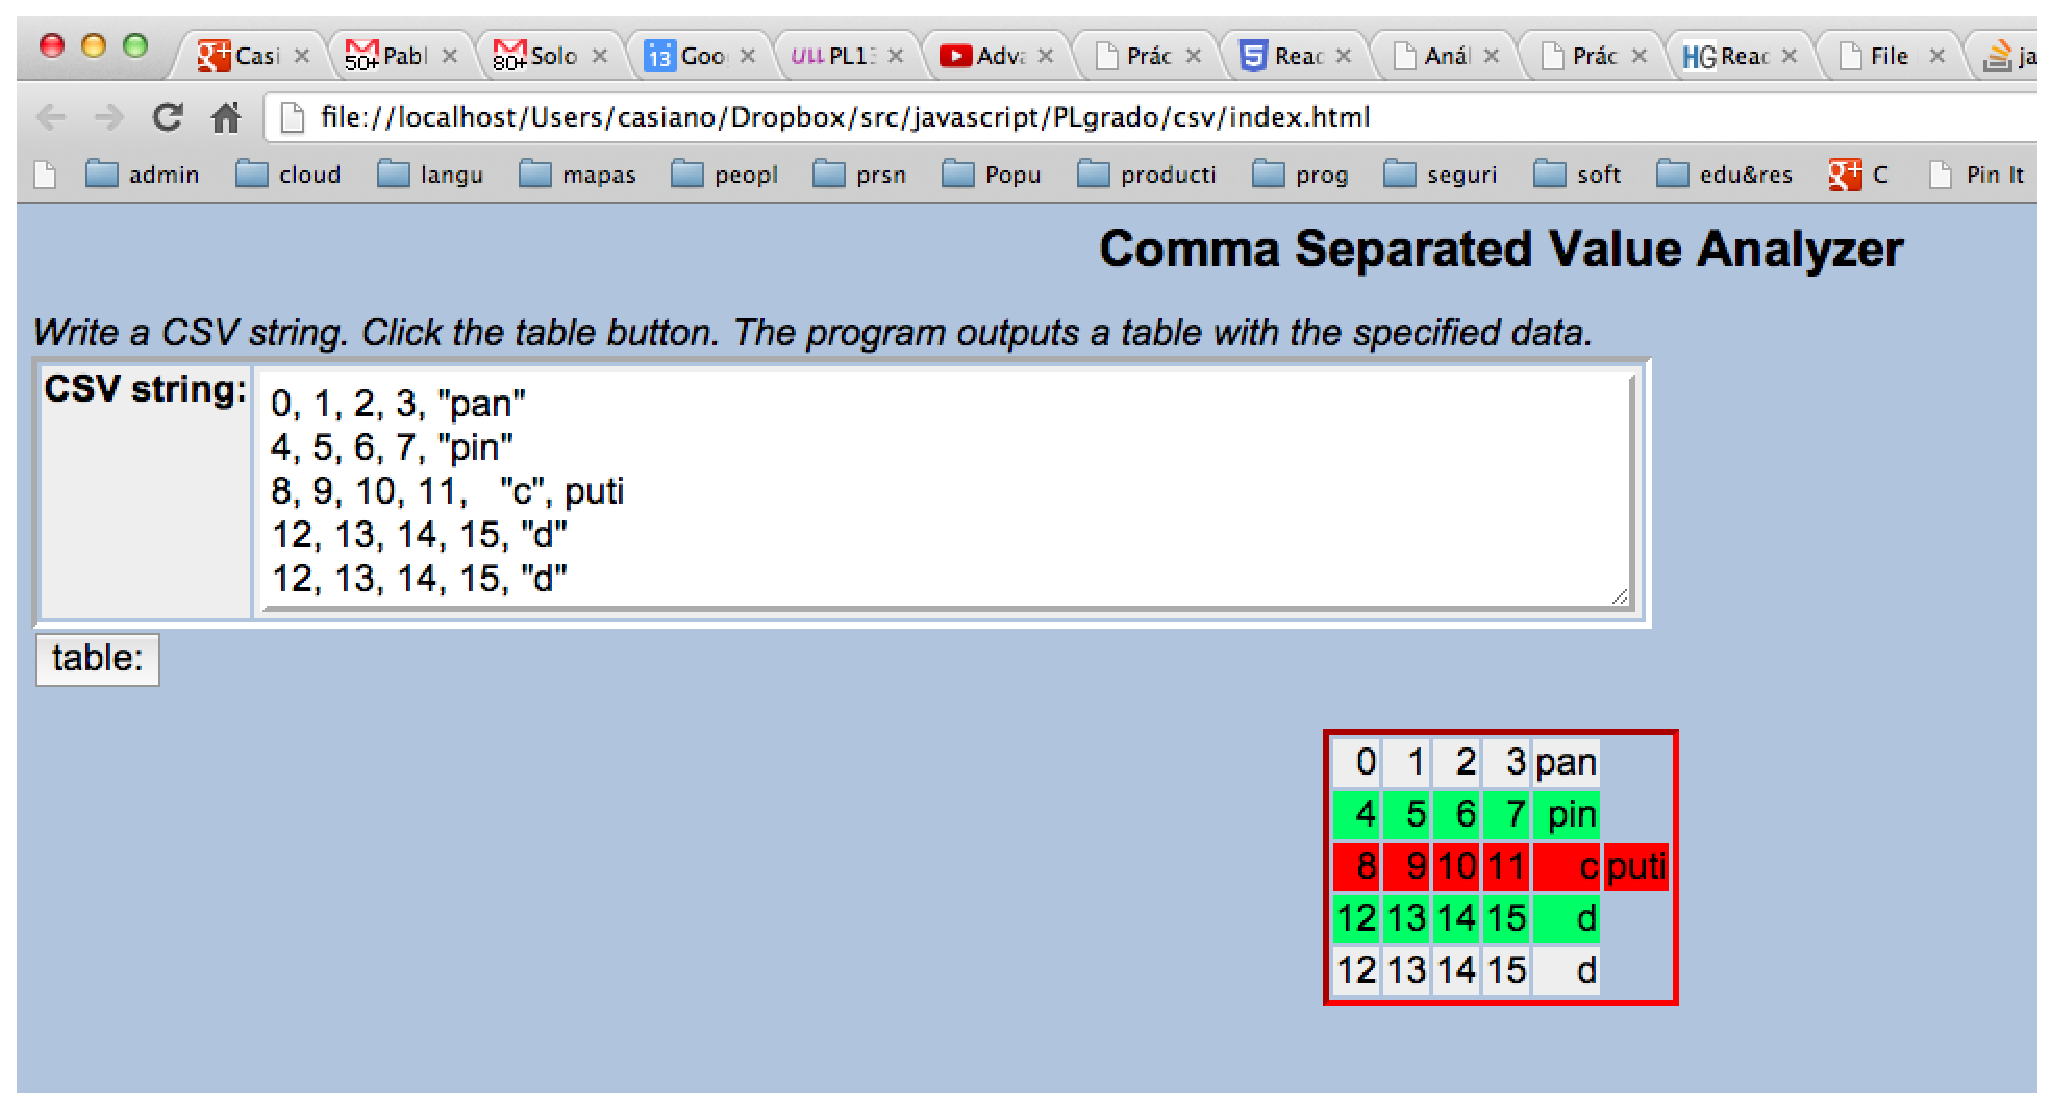
\epsfig{file=chapter2/csv.eps, width=17cm}}
\end{center}
\label{figure:csv}
\caption{Ejemplo de pantalla de La aplicación para el Análisis de Datos en Formato CSV}
\end{figure}
\end{latexonly}

\begin{rawhtml}
<DIV ALIGN="CENTER"><A NAME="figure:csv"></A><A NAME="1213"></A>
<TABLE>
<CAPTION ALIGN="BOTTOM"><STRONG>Figura:</STRONG>
Ejemplo de pantalla de La aplicación para el Análisis de Datos en Formato CSV</CAPTION>
<TR><TD><IMG
 WIDTH="769" HEIGHT="410" BORDER="0"
 SRC="csv.png"
 ALT="\begin{figure}\begin{center}
\centerline{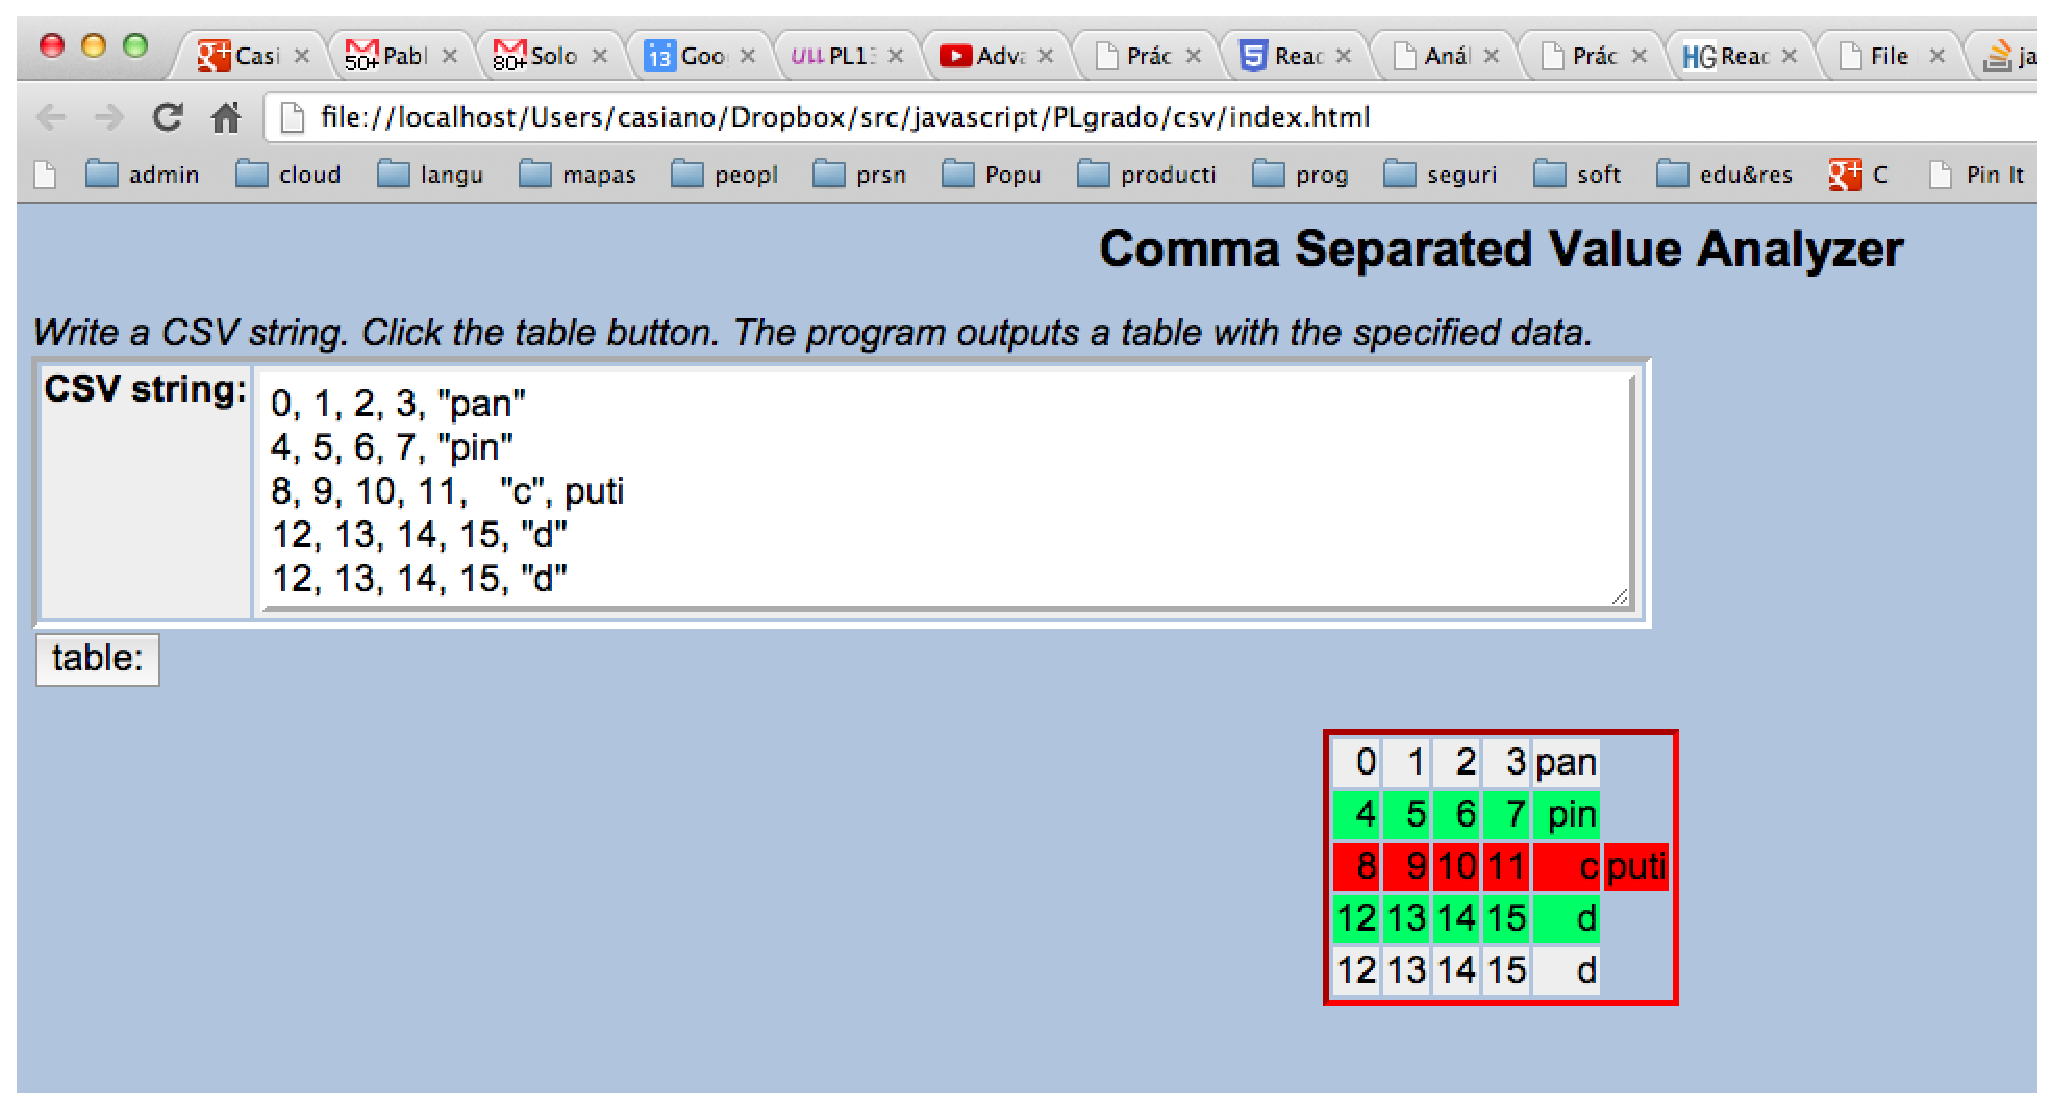
\epsfig{file=chapter2/csv.eps, width=17cm}}
\end{center}
\end{figure}"></TD></TR>
</TABLE>
</DIV>
\end{rawhtml}



\parrafo{Aproximación al análisis mediante expresiones regulares de CSV}
Una primera aproximación sería hacer \verb|split| por las comas:
\begin{verbatim}
> x = '"earth",1,"moon",9.374'
'"earth",1,"moon",9.374'
> y = x.split(/,/)
[ '"earth"', '1', '"moon"', '9.374' ]
\end{verbatim}

Esta solución deja las comillas dobles en los campos entrecomillados. 
Peor aún, los campos entrecomillados pueden contener comas, en cuyo 
caso la división proporcionada por \verb|split| sería errónea:
\begin{verbatim}
> x = '"earth, mars",1,"moon, fobos",9.374'
'"earth, mars",1,"moon, fobos",9.374'
> y = x.split(/,/)
[ '"earth', ' mars"', '1', '"moon', ' fobos"', '9.374' ]
\end{verbatim}

La siguiente expresión regular reconoce cadenas de comillas dobles
con secuencias de escape seguidas opcionalmente de una coma:
\begin{verbatim}
> x = '"earth, mars",1,"moon, fobos",9.374'
'"earth, mars",1,"moon, fobos",9.374'
> r = /"((?:[^"\\]|\\.)*)"\s*,?/g
/"((?:[^"\\]|\\.)*)"\s*,?/g
> w = x.match(r)
[ '"earth, mars",', '"moon, fobos",' ]
\end{verbatim}
If your regular expression uses the \verb"g" flag, you can use the \verb|exec| 
or \verb|match| methods
multiple times to find successive matches in the same string. When
you do so, the search starts at the substring of string specified by the
regular expression's \verb|lastIndex| property.

Javascript sub-matches stop working when the \verb|g| modifier is set:
\begin{verbatim}
> text = 'test test test test'
'test test test test'
> text.match(/t(e)(s)t/)
[ 'test', 'e', 's', index: 0, input: 'test test test test' ]
> text.match(/t(e)(s)t/g)
[ 'test', 'test', 'test', 'test' ] 
\end{verbatim}
Sin embargo el método \verb|exec| de las expresiones regulares si que 
conserva las subexpresiones que casan con los paréntesis:
\begin{verbatim}
> r = /t(e)(s)t/g
/t(e)(s)t/g
> text = 'test test test test'
'test test test test'
> while (m = r.exec(text)) {
... console.log(m);
... }
[ 'test', 'e', 's', index: 0, input: 'test test test test' ]
[ 'test', 'e', 's', index: 5, input: 'test test test test' ]
[ 'test', 'e', 's', index: 10, input: 'test test test test' ]
[ 'test', 'e', 's', index: 15, input: 'test test test test' ]
undefined
\end{verbatim}
Another catch to remember is that \verb|exec()| doesn't return the matches in
one big array: it keeps returning matches until it runs out, in which
case it returns \verb|null|.

Véase
\begin{itemize}
\item
\htmladdnormallink{Javascript Regex and Submatches}{http://stackoverflow.com/questions/844001/javascript-regex-and-submatches}
en StackOverflow.
\item
La sección 
{\it Ejercicios}
\ref{section:ejercicioslastindex}
\end{itemize}

Esta otra expresión regular \verb#/([^,]+),?|\s*,/# actúa de forma parecida al \verb|split|. 
Reconoce secuencias no vacías de caracteres que no contienen comas seguidas opcionalmente
de una coma o bien una sóla coma (precedida opcionalmente de blancos):
\begin{verbatim}
> x = '"earth, mars",1,"moon, fobos",9.374'
'"earth, mars",1,"moon, fobos",9.374'
> r = /([^,]+),?|\s*,/g
/([^,]+),?|\s*,/g
> w = x.match(r)
[ '"earth,', ' mars",', '1,', '"moon,', ' fobos",', '9.374' ]
\end{verbatim}

La siguiente expresión regular es la unión de dos: 
\begin{itemize}
\item
Cadenas de dobles comillas seguidas de una coma opcional entre espacios en blanco
\item
Cadenas que no tienen comas
\end{itemize}
\begin{verbatim}
>  x = '"earth, mars",1,"moon, fobos",9.374'
'"earth, mars",1,"moon, fobos",9.374'
> r = /\s*"((?:[^"\\]|\\.)*)"\s*,?|\s*([^,]+),?|\s*,/g
/\s*"((?:[^"\\]|\\.)*)"\s*,?|\s*([^,]+),?|\s*,/g
> w = x.match(r)
[ '"earth, mars",', '1,', '"moon, fobos",', '9.374' ]
\end{verbatim}
El operador \verb#|# trabaja en circuito corto:
\begin{verbatim}
> r = /(ba?)|(b)/
/(ba?)|(b)/
> r.exec("ba")
[ 'ba', 'ba', undefined, index: 0, input: 'ba' ]
> r = /(b)|(ba?)/
/(b)|(ba?)/
> r.exec("ba")
[ 'b', 'b', undefined, index: 0, input: 'ba' ]
\end{verbatim}

Si usamos \verb|exec| tenemos:
\begin{verbatim}
> x = '"earth, mars",1,"moon, fobos",9.374'
'"earth, mars",1,"moon, fobos",9.374'
> r = /\s*"((?:[^"\\]|\\.)*)"\s*,?|\s*([^,]+),?|\s*,/g
/\s*"((?:[^"\\]|\\.)*)"\s*,?|\s*([^,]+),?|\s*,/g
> while (m = r.exec(x)) { console.log(m); }
[ '"earth, mars",', 'earth, mars', undefined, index: 0,
  input: '"earth, mars",1,"moon, fobos",9.374' ]
[ '1,', undefined, '1', index: 14,
  input: '"earth, mars",1,"moon, fobos",9.374' ]
[ '"moon, fobos",', 'moon, fobos', undefined, index: 16,
  input: '"earth, mars",1,"moon, fobos",9.374' ]
[ '9.374', undefined, '9.374', index: 30,
  input: '"earth, mars",1,"moon, fobos",9.374' ]
undefined
\end{verbatim}


Es necesario tener en cuenta el caso de los campos vacíos, especialmente al principio y al final:
\begin{verbatim}
> w = ',"earth, mars",1,"moon,fobos",   ,9.374,'
',"earth, mars",1,"moon,fobos",   ,9.374,'
\end{verbatim}
Al analizar \verb|w| debería haber un campo vacío al principio, uno en medio
y otro al final.

Para resolverlo hemos usado lookahead \verb#(^|,)(?=\s*(,|$))# que dice que una coma seguida de una coma o el final da lugar a un nuevo campo (y que si al comienzo de la cadena 
hay una coma también se produce un nuevo campo):
\begin{verbatim}
> r
/\s*"((?:[^"\\]|\\.)*)"\s*|\s*([^,]+)|(^|,)(?=\s*(,|$))/g
> w.match(r)
[ '', '"earth, mars"', '1', '"moon,fobos"', ',', '   ', '9.374', ',' ]
\end{verbatim}

\parrafo{RegExp Objects}
\begin{enumerate}
\item \htmladdnormallink{RegExp Objects}{https://developer.mozilla.org/en-US/docs/JavaScript/Reference/Global_Objects/Regexp}

The \verb|RegExp| constructor creates a regular expression object for matching text with a pattern.

Literal and constructor notations are possible:

\begin{verbatim}
/pattern/flags; 
new RegExp(pattern [, flags]);
\end{verbatim}

\begin{itemize}
\item
The literal notation provides compilation of the regular expression
when the expression is evaluated. 

\item
Use literal notation when the regular
expression will remain constant. 

\item
For example, \red{if you use literal notation
to construct a regular expression used in a loop, the regular expression
won't be recompiled on each iteration}.
\end{itemize}

\begin{itemize}
\item
The constructor of the regular expression object, for example,
\verb|new RegExp("ab+c")|, provides runtime compilation of the regular
expression. 

\item
Use the constructor function when you know the regular
expression pattern will be changing, or you don't know the pattern and
are getting it from another source, such as user input.

\item
When using the constructor function, the normal string escape rules
(preceding special characters with \verb|\| when included in a string) are
necessary. For example, the following are equivalent:

\begin{verbatim}
var re = /\w+/;
var re = new RegExp("\\w+");
\end{verbatim}
\end{itemize}

\item 
RegExp.prototype.\htmladdnormallink{exec}{https://developer.mozilla.org/en-US/docs/JavaScript/Reference/Global_Objects/RegExp/exec}

The \verb|exec()| method executes a search for a match in a specified string. Returns a result array, or \verb|null|.

If you are executing a match simply to find \verb|true| 
or \verb1false1, 
use the \verb|RegExp.prototype.test()| method or the \verb|String.prototype.search()| method.

\item 
String.prototype.\htmladdnormallink{search}{https://developer.mozilla.org/en-US/docs/JavaScript/Reference/Global_Objects/String/search}

\verb|str.search(regexp)|

If successful, \verb|search| returns the index of the regular expression inside
the string. Otherwise, it returns \verb|-1|.

When you want to know whether a pattern is found in a string use \verb|search|
(similar to the regular expression \verb|test| method); for more information
(but slower execution) use \verb|match| (similar to the regular expression
\verb|exec| method).
\item 
String.prototype.\htmladdnormallink{match}{https://developer.mozilla.org/en-US/docs/JavaScript/Reference/Global_Objects/String/match}
\item 
String.prototype.\htmladdnormallink{replace}{https://developer.mozilla.org/en-US/docs/JavaScript/Reference/Global_Objects/String/replace}

The \verb|replace()| method returns a new string with some or all matches of
a pattern replaced by a replacement.  
The pattern can be a string or a \verb|RegExp|, 
and the replacement can be a string or a function to be called
for each match.

\begin{verbatim}
> re = /apples/gi
/apples/gi
> str = "Apples are round, and apples are juicy."
'Apples are round, and apples are juicy.'
> newstr = str.replace(re, "oranges")
'oranges are round, and oranges are juicy.'
\end{verbatim}

\red{The replacement string can be a function to be invoked to create the
new substring} (to put in place of the substring received from parameter
\verb|#1|). The arguments supplied to this function are:

\begin{tabular}{|p{5cm}|p{17cm}|}
{\bf Possible name}   & {\bf Supplied value} \\
match           & The matched substring. (Corresponds to \verb|$&|.)\\
p1, p2, ...     & The nth parenthesized submatch string, provided the first argument to replace was a RegExp object. (Corresponds to \verb|$1|, \verb|$2|, etc.) 
For example, if \verb|/(\a+)(\b+)/|, was given, p1 is the match for
\verb|\a+|, and p2 for \verb|\b+|.\\
offset          & The offset of the matched substring within the total string being examined. 
                  (For example, if the total string was \verb"abcd", and the
                  matched substring was \verb"bc", then this argument will
                  be \verb|1|.) \\
string  &The total string being examined \\
\end{tabular}

\begin{verbatim}
[~/javascript/learning]$ pwd -P
/Users/casiano/local/src/javascript/learning
[~/javascript/learning]$ cat f2c.js 
#!/usr/bin/env node
function f2c(x)
{
  function convert(str, p1, offset, s)
  {
    return ((p1-32) * 5/9) + "C";
  }
  var s = String(x);
  var test = /(\d+(?:\.\d*)?)F\b/g;
  return s.replace(test, convert);
}

var arg = process.argv[2] || "32F";
console.log(f2c(arg));
\end{verbatim}

\begin{verbatim}
[~/javascript/learning]$ ./f2c.js 100F
37.77777777777778C
[~/javascript/learning]$ ./f2c.js 
0C
\end{verbatim}
\end{enumerate}


\parrafo{index.html}
Los dos hechos mas relevantes en este \verb|index.html| son el uso de las librerías 
\verb|jquery|, \verb|underscore| y el uso de un elemento \verb|textarea| en vez de un \verb|input| para la entrada:
\begin{verbatim}
<html>
  <head>
     <meta http-equiv="Content-Type" content="text/html; charset=UTF-8">
     <title>CSV Analyzer</title>
     <link href="global.css" rel="stylesheet" type="text/css">

     <script type="text/javascript" src="../../underscore/underscore.js"></script>
     <script type="text/javascript" src="../../jquery/starterkit/jquery.js"></script>
     <script type="text/javascript" src="csv.js"></script>
  </head>
  <body>
    <h1>Comma Separated Value Analyzer</h1>
    <div>
      <i>Write a CSV string. Click the table button. The program outputs a table with the specified data.</i>
    </div>
    <table>
      <tr>
        <th>CSV string:</th> <!-- autofocus attribute is HTML5 -->
        <td><textarea autofocus cols = "80" rows = "5" id="original"></textarea></td> 
      </tr>
    </table>
    <button type="button">table:</button><br>
    <span class="output" id="finaltable"></span>
  </body>
</html>
\end{verbatim}

%\parrafos separados
\parrafo{jQuery}

\htmladdnormallink{jQuery}{http://jquery.com/} (\htmladdnormallink{Descarga la librería}{http://jquery.com/download/})

\cei{jQuery} is a cross-platform JavaScript library designed to simplify
the client-side scripting of HTML. 

\begin{itemize}
\item
It was released in January 2006
at BarCamp NYC by John Resig. 

\item
It is currently developed by a team of
developers led by Dave Methvin. 

\item
jQuery is the most popular JavaScript library in
use today

\item
jQuery's syntax is designed to make it easier 
\begin{itemize}
\item
to navigate a document,
\item
select DOM elements, 
\item
create animations, 
\item
handle events, and 
\item
develop Ajax applications. 
\end{itemize}

\item
The set of jQuery core features — DOM element selections, traversal
and manipulation — enabled by its selector engine (named "Sizzle"
from v1.3), created a new "programming style", fusing algorithms and
DOM-data-structures; and influenced the architecture of other JavaScript
frameworks like \wikip{YUI v3}{YUI\_Library} and \wikip{Dojo}{Dojo\_Toolkit}.
\item
\end{itemize}

\parrafo{How JQuery Works}

  \begin{itemize}
  \item
  Véase
  \htmladdnormallink{How jQuery Works}{http://learn.jquery.com/about-jquery/how-jquery-works/}
  \item
    \htmladdnormallink{https://github.com/crguezl/how-jquery-works-tutorial}{https://github.com/crguezl/how-jquery-works-tutorial} en GitHub
  \item
  \begin{verbatim}
  [~/javascript/jquery(master)]$ pwd -P
  /Users/casiano/local/src/javascript/jquery
  \end{verbatim}
  \item \htmladdnormallink{w3schools JQuery tutorial}{http://www.w3schools.com/jquery/default.asp}
  \end{itemize}

\begin{verbatim}
~/javascript/jquery(master)]$ cat index.html 
<!doctype html>
<html>
<head>
    <meta charset="utf-8" />
    <title>Demo</title>
</head>
<body>
    <a href="http://jquery.com/">jQuery</a>
    <script src="starterkit/jquery.js"></script>
    <script>
 
    // Your code goes here.
 
    </script>
</body>
</html>
\end{verbatim}

To ensure that their code runs after the browser finishes loading the document, many JavaScript programmers wrap their code in an onload function:

\begin{verbatim}
window.onload = function() { alert( "welcome" ); }
\end{verbatim}

Unfortunately, the code doesn't run until all images are finished downloading, including banner ads. To run code as soon as the document is ready to be manipulated, jQuery has a statement known as the ready event:

\begin{verbatim}
$( document ).ready(function() {
    // Your code here.
});
\end{verbatim}
For \verb|click| and most other events, you can prevent the default
behavior by calling 
\htmladdnormallink{event.preventDefault()}{http://api.jquery.com/event.preventdefault/}
in the event handler.
If this method is called, the default action of the event will not be triggered.
For example, clicked anchors will not take the browser to a new URL.

\begin{verbatim}
[~/javascript/jquery(master)]$ cat index2.html 
<!doctype html>
<html>
<head>
    <meta charset="utf-8" />
    <title>Demo</title>
</head>
<body>
    <a href="http://jquery.com/">jQuery</a>
    <script src="starterkit/jquery.js"></script>
    <script>
 
    $( document ).ready(function() {
        $( "a" ).click(function( event ) {
            alert( "The link will no longer take you to jquery.com" );
            event.preventDefault();
        });
    });
 
    </script>
</body>
</html>
\end{verbatim}
Borrowing from CSS 1–3, and then adding its own, jQuery offers a powerful set of tools for matching a set of elements in a document.

See jQuery \htmladdnormallink{Category: Selectors}{http://api.jquery.com/category/selectors/}.

Another common task is adding or removing a class.
jQuery also provides some handy effects.

\begin{verbatim}
[~/javascript/jquery(master)]$ cat index3.html 
<!doctype html>
<html>
<head>
    <meta charset="utf-8" />
    <style>
        a.test { font-weight: bold; }
    </style>
    <title>Demo</title>
</head>
<body>
    <a href="http://jquery.com/">jQuery</a>
    <script src="starterkit/jquery.js"></script>
    <script>
 
    $( document ).ready(function() {
        $( "a" ).click(function( event ) {
            $( "a" ).addClass( "test" );
            alert( "The link will no longer take you to jquery.com" );
            event.preventDefault();
            $( "a" ).removeClass( "test" );
            $( this ).hide( "slow" );
            $( this ).show( "slow" );
        });
    });
 
    </script>
</body>
</html>
\end{verbatim}
\begin{itemize}
\item
In JavaScript \verb|this| always refers to the {\it owner} of the function
we're executing, or rather, {\it to the object that a function is a method of}.

\item
When we define our function \verb|tutu()| in a page, its owner is the
page, or rather, the \verb|window| object (or \verb|global| object) of JavaScript. 

\item
An \verb|onclick| property, though, is owned by the HTML element it belongs to.

\item
The method
\htmladdnormallink{.addClass( className )}{http://api.jquery.com/addclass/}
adds the specified class(es) to each of the set of matched elements.

\verb|className| is a String containing 
one or more space-separated classes to be added to the class attribute of each matched element.

This method does not replace a class. It simply adds the class, appending
it to any which may already be assigned to the elements.
\item
The method \verb|.removeClass( [className ] )|
removes a single class, multiple classes, or all classes from each element in the set of matched elements.

If a class name is included as a parameter, then only that class will be
removed from the set of matched elements. If no class names are specified
in the parameter, all classes will be removed.

This method is often used with \verb|.addClass()| 
to switch elements' classes from one to another, like so:

\begin{verbatim}
$( "p" ).removeClass( "myClass noClass" ).addClass( "yourClass" );
\end{verbatim}

\end{itemize}


\parrafo{Ejemplo usando Ajax con jQuery y Express.js}

\htmladdnormallink{Código del server}{https://github.com/crguezl/how-jquery-works-tutorial/tree/getallparams}:

\begin{verbatim}
[~/javascript/jquery/how-jquery-works-tutorial(getallparams)]$ cat app.js
var express = require('express');
var app = express();
var path = require('path');

app.use(express.static('public'));

// view engine setup
app.set('views', path.join(__dirname, 'views'));
app.set('view engine', 'ejs');

app.get('/', function (req, res) {
  res.render('index', { title: 'Express' });
})

app.get('/chuchu', function (req, res) {
  var isAjaxRequest = req.xhr;
  console.log(isAjaxRequest);
  if (isAjaxRequest) {
    console.log(req.query);
    res.send('{"answer": "Server responds: hello world!"}')
  }
  else {
    res.send('not an ajax request');
  }
});

var server = app.listen(3000, function () {

  var host = server.address().address
  var port = server.address().port

  console.log('Example app listening at http://%s:%s', host, port)

});
\end{verbatim}

\begin{itemize}
\item \verb|jQuery.get( url [, data ] [, success(data, textStatus, jqXHR) ] [, dataType ] )|
load data from the server using a HTTP GET request.

\item \verb|url|

Type: String

A string containing the URL to which the request is sent.
\item \verb|data|

Type: PlainObject or String

A plain object or string that is sent to the server with the request.
\item \verb|success(data, textStatus, jqXHR)|

Type: Function()

A callback function that is executed if the request succeeds.
\item \verb|dataType|

Type: String

The type of data expected from the server. Default: Intelligent Guess 
(\verb|xml|, \verb|json|, \verb|script|, \verb|or| \verb|html|).
\end{itemize}

To use callbacks, it is important to know how to pass them into their parent function.

En el directorio \verb|views| hemos puesto el template:
\begin{verbatim}
[~/javascript/jquery/how-jquery-works-tutorial(getallparams)]$ cat views/index.ejs 
<!doctype html>
<html>
  <head>
    <title><%- title %></title>
  </head>
  <body>
    <h1><%- title  %></h1>
    <ul>
      <li><a href="http://jquery.com/" id="jq">jQuery</a>
      <li><a href="/chuchu">Visit chuchu!</a>
    </ul>
    <div class="result"></div>
    <script src="https://code.jquery.com/jquery-2.1.3.js"></script>
    <script>
      $( document ).ready(function() {
          $( "#jq" ).click(function( event ) {
              event.preventDefault();
              $.get( "/chuchu", {nombres: ["juan", "pedro"]}, function( data ) {
                $( ".result" ).html( data["answer"]);
                console.log(data);
              }, 'json');
          });
      });
    </script>
  </body>
</html>
\end{verbatim}
\begin{itemize}
\item
\verb|req.query|

An object containing a property for each query string parameter in the route. If there is no query string, it is the empty object, \verb|{}|.

\begin{verbatim}
// GET /search?q=tobi+ferret
req.query.q
// => "tobi ferret"

// GET /shoes?order=desc&shoe[color]=blue&shoe[type]=converse
req.query.order
// => "desc"

req.query.shoe.color
// => "blue"

req.query.shoe.type
// => "converse"
\end{verbatim}
\end{itemize}

Estas son las dependencias:
\begin{verbatim}
[~/javascript/jquery/how-jquery-works-tutorial(getallparams)]$ cat package.json 
{
  "name": "ajaxjquery",
  "version": "0.0.0",
  "description": "",
  "main": "hello.js",
  "dependencies": {
    "express": "*",
    "ejs": "*",
    "gulp-shell": "*",
    "body-parser": "~1.12.0"
  },
  "devDependencies": {},
  "scripts": {
    "test": "node hello.js"
  },
  "author": "",
  "license": "ISC"
}
\end{verbatim}
Además hemos instalado a nivel global \verb|gulp| y \verb|node-supervisor|.

Podemos arrancar el servidor usando este \verb|gulpfile|:

\begin{verbatim}
[~/javascript/jquery/how-jquery-works-tutorial(getallparams)]$ cat gulpfile.js 
var gulp    = require('gulp');
var shell = require('gulp-shell');

gulp.task('default', ['server']);

// npm install supervisor -g
gulp.task('server', function () {
  return gulp.src('').pipe(shell([ 'node-supervisor app.js' ]));
});

gulp.task('open', function() {
  return gulp.src('').
           pipe(shell("open https://github.com/crguezl/how-jquery-works-tutorial/tree/getallparams"));
});
\end{verbatim}

\parrafo{Ejemplo de como Desplegar una Aplicación  Express sobre Node.JS en Heroku}

Véase:
\begin{itemize}
\item
La rama heroku del repo \htmladdnormallink{how-jquery-works-tutorial}{https://github.com/crguezl/how-jquery-works-tutorial/tree/heroku}
\item
El tutorial de Heroku 
\htmladdnormallink{Getting Started with Node.js on Heroku}{https://devcenter.heroku.com/articles/getting-started-with-nodejs}
\item
El capítulo sobre Heroku en los apuntes de LPP
\end{itemize}



\parrafo{Ajax, jQuery y Sinatra}

JavaScript enables you to freely
pass functions around to be executed at a later time. A \cei{callback} is a
function that is passed as an argument to another function and is usually 
executed
after its parent function has completed. 

Callbacks are special because
they wait to execute until their parent finishes or some event occurs. 

Meanwhile, the
browser can be executing other functions or doing all sorts of other work.
\begin{verbatim}
[~/javascript/jquery(master)]$ cat app.rb
require 'sinatra'

set :public_folder, File.dirname(__FILE__) + '/starterkit'

get '/' do
  erb :index
end

get '/chuchu' do
  if request.xhr?
    "hello world!"
  else 
    erb :tutu
  end
end

__END__

@@layout
  <!DOCTYPE html>
  <html>
    <head>
        <meta charset="utf-8" />
        <title>Demo</title>
    </head>
    <body>
        <a href="http://jquery.com/">jQuery</a>
        <div class="result"></div>
        <script src="jquery.js"></script>
        <%= yield %>
    </body>
  </html>

@@index
  <script>
  $( document ).ready(function() {
      $( "a" ).click(function( event ) {
          event.preventDefault();
          $.get( "/chuchu", function( data ) {
            $( ".result" ).html( data );
            alert( "Load was performed." );
          });
      });
  });
  </script>

@@tutu
  <h1>Not an Ajax Request!</h1>
\end{verbatim}

\begin{itemize}
\item \verb|jQuery.get( url [, data ] [, success(data, textStatus, jqXHR) ] [, dataType ] )|
load data from the server using a HTTP GET request.

\item \verb|url|

Type: String

A string containing the URL to which the request is sent.
\item \verb|data|

Type: PlainObject or String

A plain object or string that is sent to the server with the request.
\item \verb|success(data, textStatus, jqXHR)|

Type: Function()

A callback function that is executed if the request succeeds.
\item \verb|dataType|

Type: String

The type of data expected from the server. Default: Intelligent Guess 
(\verb|xml|, \verb|json|, \verb|script|, \verb|or| \verb|html|).
\end{itemize}

To use callbacks, it is important to know how to pass them into their parent function.


Executing callbacks with arguments can be tricky.

This code example will not work:

\begin{verbatim}
$.get( "myhtmlpage.html", myCallBack( param1, param2 ) );
\end{verbatim}
The reason this fails is that the code executes 

\begin{verbatim}
myCallBack( param1, param2) 
\end{verbatim}

immediately and then passes \verb|myCallBack()|'s return value as the second
parameter to \verb|$.get()|. 

We actually want to pass the function \verb|myCallBack|,
not \verb|myCallBack( param1, param2 )|'s return value (which might or might not
be a function). 

So, how to pass in \verb|myCallBack()| and include arguments?

To defer executing \verb|myCallBack()| with its parameters, you can use
an anonymous function as a wrapper.


\begin{verbatim}
[~/javascript/jquery(master)]$ cat app2.rb
require 'sinatra'

set :public_folder, File.dirname(__FILE__) + '/starterkit'

get '/' do
  erb :index
end

get '/chuchu' do
  if request.xhr? # is an ajax request
    "hello world!"
  else 
    erb :tutu
  end
end

__END__

@@layout
  <!DOCTYPE html>
  <html>
    <head>
        <meta charset="utf-8" />
        <title>Demo</title>
    </head>
    <body>
        <a href="http://jquery.com/">jQuery</a>
        <div class="result"></div>
        <script src="jquery.js"></script>
        <%= yield %>
    </body>
  </html>

@@tutu
  <h1>Not an Ajax Request!</h1>

@@index
  <script>
    var param = "chuchu param";
    var handler = function( data, textStatus, jqXHR, param ) {
      $( ".result" ).html( data );
      alert( "Load was performed.\n"+
             "$data = "+data+
             "\ntextStatus = "+textStatus+
             "\njqXHR = "+JSON.stringify(jqXHR)+
             "\nparam = "+param );
    };
    $( document ).ready(function() {
        $( "a" ).click(function( event ) {
            event.preventDefault();
            $.get( "/chuchu", function(data, textStatus, jqXHR ) {
              handler( data, textStatus, jqXHR, param);
            });
        });
    });
  </script>
\end{verbatim}
El ejemplo en \verb|app2.rb| puede verse desplegado en Heroku:
\htmladdnormallink{http://jquery-tutorial.herokuapp.com/}{http://jquery-tutorial.herokuapp.com/}







\parrafo{JSON.stringify()}
\label{parrafo:jsonstringify}
The
\htmladdnormallink{JSON.stringify() }{https://developer.mozilla.org/en-US/docs/Web/JavaScript/Reference/Global_Objects/JSON/stringify}
method converts a value to \tei{JSON}, optionally replacing values
if a \verb|replacer function| is specified, or optionally including only the
specified properties if a \verb|replacer array| is specified.

\verb|JSON.stringify(value[, replacer [, space]])|
\begin{itemize}
\item
\verb|value|

The value to convert to a JSON string.
\item
\verb|replacer|

  \begin{itemize}
  \item
  If a function, transforms values and properties encountered while stringifying; 
  \item
  if an array, specifies the set of properties included in objects in the final string.
  \end{itemize}

\item
\verb|space|

Causes the resulting string to be pretty-printed.
\end{itemize}


See another example of use in
\htmladdnormallink{http://jsfiddle.net/casiano/j7tsF/}{http://jsfiddle.net/casiano/j7tsF/}.
To learn to use JSFiddle wath the YouTube video 
\htmladdnormallink{How to use JSFiddle by Jason Diamond}{http://youtu.be/Iw4f-yRf7RU}




\parrafo{Underscore}

\htmladdnormallink{Underscore}{http://underscorejs.org/}:
is a utility-belt library for JavaScript that provides a
lot of the functional programming support that you would expect in
Ruby.

\begin{itemize}
\item
Underscore provides functions that support 
methods like: 

\verb|map|, \verb|select|, \verb|invoke|  

\item
as well as more specialized helpers:

En ECMAScript 5/JavaScript 1.6.  existen los métodos 
\verb|map|, \verb|filter|, \verb|forEach| y  \verb|reduce| similares
a los de Underscore.

\begin{itemize}
\item
function binding
\item
 javascript templating
\item
 deep equality testing
\item
 and so on. 
\end{itemize}

\begin{itemize}
\item
Cargando la librería:
\begin{verbatim}
[~/javascript/jquery(master)]$ node
> 2+3
5
> _
5
> uu = require('underscore')
{ [Function]
  _: [Circular],
  VERSION: '1.5.2',
  forEach: [Function],
  each: [Function],
  collect: [Function],
  map: [Function],
  inject: [Function],
  reduce: [Function],
  .................
  chain: [Function] }
\end{verbatim}

\item \verb|each|:

\begin{verbatim}
> uu.each([1, 2, 3], function(x) { console.log(x*x); })
1
4
9
\end{verbatim}

\item
\verb|map|:
\begin{verbatim}
> uu.map([1, 2, 3], function(num){ return num * 3; })
[ 3, 6, 9 ]
\end{verbatim}
\item \verb|invoke|
\begin{verbatim}
> z = [[6,9,1],[7,3,9]]
[ [ 6, 9, 1 ], [ 7, 3, 9 ] ]
> uu.invoke(z, 'sort')
[ [ 1, 6, 9 ], [ 3, 7, 9 ] ]
> uu.invoke(z, 'sort', function(a, b) { return b-a; })
[ [ 9, 6, 1 ], [ 9, 7, 3 ] ]
\end{verbatim}
\item
\verb|reduce|:
\begin{verbatim}
> uu.reduce([1, 2, 3, 4], function(s, num){ return s + num; }, 0)
10
> uu.reduce([1, 2, 3, 4], function(s, num){ return s * num; }, 1)
24
> uu.reduce([1, 2, 3, 4], function(s, num){ return Math.max(s, num); }, -1)
4
> uu.reduce([1, 2, 3, 4], function(s, num){ return Math.min(s, num); }, 99)
1
\end{verbatim}

\item \verb|filter|: (\verb|select| is an alias for \verb|filter|)
\begin{verbatim}
> uu.filter([1, 2, 3, 4, 5, 6], function(num){ return num % 2 == 0; })
[ 2, 4, 6 ]
\end{verbatim}
\item \verb|isEqual|
\begin{verbatim}
> a = {a:[1,2,3], b: { c: 1, d: [5,6]}}
{ a: [ 1, 2, 3 ],
  b: { c: 1, d: [ 5, 6 ] } }
> b = {a:[1,2,3], b: { c: 1, d: [5,6]}}
{ a: [ 1, 2, 3 ],
  b: { c: 1, d: [ 5, 6 ] } }
> a == b
false
> uu.isEqual(a,b)
true
\end{verbatim}
\item \verb|bind|
\begin{verbatim}
> func = function(greeting){ return greeting + ': ' + this.name }
[Function]
> func = uu.bind(func, {name: 'moe'})
[Function]
> func('hello')
'hello: moe'
> func = uu.bind(func, {name: 'moe'}, 'hi')
[Function]
> func()
'hi: moe'
> 
\end{verbatim}
Los objetos \verb|Function| disponen de un método \verb|bind|
nativo en las últimas versiones de JS:
\begin{verbatim}
> func = function(){ return 'hola ' + this.name }
[Function]
> g = func.bind({name: 'Juan'})
[Function]
> g()
'hola Juan'
> g = func.bind({name: 'Pedro'})
[Function]
> g()
'hola Pedro'
\end{verbatim}
\end{itemize}
\end{itemize}

\parrafo{Templates en Underscore}

\begin{itemize}
\item 
\htmladdnormallink{Underscore: template}{http://underscorejs.org/\#template}

\verb|_.template(templateString, [data], [settings])|

Compiles JavaScript templates into functions that can be evaluated for
rendering. Useful for rendering complicated bits of HTML from a JavaScript 
object or from \cei{JSON} data
sources.

JSON, or \cei{JavaScript Object Notation}, is an open standard format
that uses human-readable text to transmit data objects consisting of
attribute–value pairs. It is used primarily to transmit data between
a server and web application, as an alternative to XML.
Although originally derived from the JavaScript scripting language,
JSON is a language-independent data format, and code for parsing
and generating JSON data is readily available in a large variety of
programming languages.

\begin{itemize}
\item
Template functions can both interpolate variables, using 
\verb|<%= … %>|, 

\begin{verbatim}
> compiled = uu.template("hello: <%= name %>")
{ [Function]
  source: 'function(obj){
    var __t,__p=\'\', __j=Array.prototype.join, i
        print=function(){__p+=__j.call(arguments,\'\');};
    with(obj||{}){
      __p+=\'hello: \'+ ((__t=( name ))==null?\'\':__t)+ \'\';
    }
    return __p;
  }' 
}
> compiled({name: 'moe'})
'hello: moe'
\end{verbatim}
\item
as well as execute arbitrary JavaScript code, with 
\verb|<% … %>|. 

\begin{verbatim}
> uu = require('underscore')
> list = "\
... <% _.each(people, function(name) { %>\
..... <li><%= name %></li>\
... <% }); %>"
'<% _.each(people, function(name) { %> <li><%= name %></li> <% }); %>'
> uu.template(list, {people: ['moe', 'curly', 'larry']})
' <li>moe</li>  <li>curly</li>  <li>larry</li> '
\end{verbatim}

\item
When you evaluate a template function, pass in a data object
that has properties corresponding to the template's free variables. 

\item
If
you're writing a one-off, like in the example above, 
you can pass the data object as the second
parameter to template in order to render immediately instead of returning
a template function 
\begin{verbatim}
> uu.template("hello: <%= name %>", { name: 'Mary'})
'hello: Mary'
\end{verbatim}
\item
If
you wish to interpolate a value, and have it be HTML-escaped, use 
\verb|<%- … %>| 

\begin{verbatim}
> template = uu.template("<b><%- value %></b>")
{ [Function]
  source: 'function(obj){
    var __t,__p=\'\',__j=Array.prototype.join,print=function(){__p+=__j.call(arguments,\'\');};
    with(obj||{}){
      __p+=\'<b>\'+
      ((__t=( value ))==null?\'\':_.escape(__t))+
      \'</b>\';
    }
    return __p;
  }' 
}
> template({value: '<script>'})
'<b>&lt;script&gt;</b>'
\end{verbatim}

\item
The \verb|settings| argument should be a hash containing
any \verb|_.templateSettings| that should be overridden.
\begin{verbatim}
_.template("Using 'with': <%= data.answer %>", {answer: 'no'}, {variable: 'data'});
=> "Using 'with': no"
\end{verbatim}
Another example:
\begin{verbatim}
template = uu.template("<b>{{ value }}</b>",{value: 4 },
                      { interpolate: /\{\{(.+?)\}\}/g })
'<b>4</b>'
\end{verbatim}
\end{itemize}

You can also use \verb|print| from within JavaScript code. This is sometimes
more convenient than using \verb|<%= ... %>|.

\begin{verbatim}
> compiled = uu.template("<% print('Hello ' + epithet); %>")
{ [Function]
  source: 'function(obj){\n
    var __t,__p=\'\',
        __j=Array.prototype.join,print=function(){
            __p+=__j.call(arguments,\'\');};\n
            with(obj||{}){\n
              __p+=\'\';\n print(\'Hello \' + epithet); \n
              __p+=\'\';\n}\n
              return __p;\n
  }' 
}
> compiled({ epithet : 'stooge' })
'Hello stooge'
> 
\end{verbatim}

If ERB-style delimiters aren't your cup of tea, you can change
Underscore's template settings to use different symbols to set off
interpolated code: 

\begin{itemize}
\item
Define an \verb|interpolate| regex to match expressions that
should be interpolated verbatim, 
\item
an \verb|escape| regex to match expressions
that should be inserted after being HTML escaped, and 
\item
an \verb|evaluate| regex
to match expressions that should be evaluated without insertion into
the resulting string. 
\item
You may define or omit any combination of the
three. 
\item
For example, to perform \verb|Mustache.js| style templating:

\begin{verbatim}
_.templateSettings = {
  interpolate: /\{\{(.+?)\}\}/g
};

var template = _.template("Hello {{ name }}!");
template({name: "Mustache"});
=> "Hello Mustache!"
\end{verbatim}
\item \verb|escape|:
\begin{verbatim}
> uu.templateSettings.escape = /\{\{-(.*?)\}\}/g
/\{\{-(.*?)\}\}/g
> compiled = uu.template("Escaped: {{- value }}\nNot escaped: {{ value }}")
{ [Function]
  source: 'function(obj){\nvar __t,__p=\'\',__j=Array.prototype.join,print=function(){__p+=__j.call(arguments,\'\');};\nwith(obj||{}){\n__p+=\'Escaped: \'+\n((__t=( value ))==null?\'\':_.escape(__t))+\n\'\\nNot escaped: {{ value }}\';\n}\nreturn __p;\n}' }
> compiled({value: 'Hello, <b>world!</b>'})
'Escaped: Hello, &lt;b&gt;world!&lt;/b&gt;\nNot escaped: {{ value }}'
\end{verbatim}
\item Another example:
\begin{verbatim}
> uu.templateSettings = {
.....       interpolate: /\<\@\=(.+?)\@\>/gim,
.....       evaluate: /\<\@(.+?)\@\>/gim
.....   }
{ interpolate: /\<\@\=(.+?)\@\>/gim,
  evaluate: /\<\@(.+?)\@\>/gim }
> s = " <@ _.each([0,1,2,3,4], function(i) { @>  <p><@= i @></p> <@ }); @>"
' <@ _.each([0,1,2,3,4], function(i) { @>  <p><@= i @></p> <@ }); @>'
> uu.template(s,{})
'   <p>0</p>   <p>1</p>   <p>2</p>   <p>3</p>   <p>4</p> '
\end{verbatim}
\end{itemize}
By default, template places the values from your data in the local scope
via the \verb|with| statement. The \verb'with' statement adds the given
object to the head of this scope chain during the evaluation of its
statement body:
\begin{verbatim}
> with (Math) {
... s = PI*2;
... }
6.283185307179586
> z = { x : 1, y : 2 }
{ x: 1, y: 2 }
> with (z) {
... console.log(y);
... }
2
undefined
\end{verbatim}

However, you can specify a single variable name
with the variable \verb|setting|. This improves the speed at
which a template is able to render.

\begin{verbatim}
_.template("Using 'with': <%= data.answer %>", {answer: 'no'}, {variable: 'data'});
=> "Using 'with': no"
\end{verbatim}


\item
\htmladdnormallink{JSFIDDLE: underscore templates}{http://jsfiddle.net/casiano/LS384/}
\item 
\htmladdnormallink{Stackoverflow::how to use Underscore template}{http://stackoverflow.com/questions/4778881/how-to-use-underscore-js-as-a-template-engine}

\end{itemize}




\parrafo{Content delivery network or content distribution network (CDN)}

Una CDN que provee \verb|underscore| esta en 
\htmladdnormallink{http://cdnjs.com/}{http://cdnjs.com/}:
\begin{verbatim}
<script type="text/javascript" src="https://cdnjs.cloudflare.com/ajax/libs/underscore.js/1.5.2/underscore-min.js"></script>
<script src="https://ajax.googleapis.com/ajax/libs/jquery/1.10.2/jquery.min.js"></script>
\end{verbatim}

A content delivery network or content distribution network (CDN) is a
large distributed system of servers deployed in multiple data centers
across the Internet. The goal of a CDN is to serve content to end-users
with high availability and high performance. CDNs serve a large fraction
of the Internet content today, including 
\begin{itemize}
\item
web objects (text, graphics and scripts), 
\item
downloadable objects (media files, software, documents), applications (e-commerce, portals), 
\item
live streaming media, on-demand
streaming media, and social networks.
\end{itemize}

Google provee también un servicio CDN para los desarrolladores en
\htmladdnormallink{https://developers.google.com/speed/libraries/devguide}{https://developers.google.com/speed/libraries/devguide}.


\parrafo{textarea, autofocus y button}
\begin{enumerate}

\item \htmladdnormallink{textarea}{http://www.w3schools.com/tags/tag_textarea.asp}:

The \verb|<textarea>| tag defines a multi-line text input control.

A \cei{text area} can hold an unlimited number of characters, and the text
renders in a fixed-width font (usually Courier).

The size of a text area can be specified by the \verb|cols| and \verb|rows| 
attributes, or through CSS' \verb|height| and \verb|width| properties.

\verb|cols| and \verb|rows| consider the font size. 
\verb|height| and \verb|width| aren't.

\item \htmladdnormallink{autofocus}{http://www.w3api.com/wiki/HTML5:INPUT.autofocus}.

The autofocus attribute is a boolean attribute.

When present, it specifies that the text area should automatically get focus when the page loads.

Véase también \cite{pilgrimhtml5}

\item \htmladdnormallink{button}{http://www.w3schools.com/tags/tag_button.asp}:

The \verb|<button>| tag defines a clickable button.

Inside a \verb|<button>| element you can put content, like text or images. 

\end{enumerate}

% \parrafo{Local Storage (HTML5 Web Storage)}
\parrafo{Local Storage (HTML5 Web Storage)}

\cei{Web storage} and \cei{DOM storage} 
(document object model) are web application
software methods and protocols used for storing data in a web browser. 

\begin{itemize}
\item
Web storage supports persistent data storage, similar to cookies but with
a greatly enhanced capacity and no information stored in the HTTP
request header.

\item
Local Storage nos permite almacenar hasta 5MB del lado del cliente
por dominio, esto nos permite ahora hacer aplicaciones mas robustas y
con mas posibilidades. Las Cookies ofrecen algo
parecido, pero con el limite de 100kb.

\item
There are two main web storage types: \cei{local storage}
and \cei{session storage}, behaving similarly to persistent cookies and session
cookies respectively.
\item
Unlike cookies, which can be accessed by both the server and client side, web storage falls exclusively under the purview of client-side scripting
\item
The HTML5 localStorage object is isolated per domain (the same segregation rules as the \wikip{same origin policy}{Same\_origin\_policy}).
Under this policy, \blue{a web browser permits scripts contained in a first web page to access data in a second web page, but only if both web pages have the same origin}. 

The same-origin policy \red{permits scripts running on pages originating from the same
site} – \blue{a combination of scheme, hostname, and port number} – \red{to access
each other's DOM with no specific restrictions}, {\bf but prevents access to
DOM on different sites}.
\end{itemize}

Véase:
\begin{itemize}
\item
Ejemplo en  GitHub:
\htmladdnormallink{https://github.com/crguezl/web-storage-example}{https://github.com/crguezl/web-storage-example}
\begin{verbatim}
[~/javascript/local_storage(master)]$ pwd -P
/Users/casiano/local/src/javascript/local_storage
\end{verbatim}
\item 
\htmladdnormallink{Como usar localstorage}{http://html5facil.com/tutoriales/como-usar-local-storage-de-javascript}

\item 
\htmladdnormallink{HTML5 Web Storage}{http://www.w3schools.com/html/html5_webstorage.asp}
\item
\htmladdnormallink{W3C Web Storage}{http://www.w3.org/TR/webstorage/}
\item
\htmladdnormallink{Using HTML5 localStorage To Store JSON}{http://getfishtank.ca/blog/using-html5-localstorage-to-store-json}
Options for persistent storage of complex JavaScript objects in HTML5
by Dan Cruickshank
\item
\htmladdnormallink{HTML5 Cookbook.  Christopher Schmitt, Kyle Simpson "O'Reilly Media, Inc.", Nov 7, 2011}{http://books.google.es/books/about/HTML5_Cookbook.html?id=cXcaY7XVZbcC&redir_esc=y}
Chapter 10. Section 2: LocalStorage
\end{itemize}

While Chrome does not provide a UI for clearing localStorage, there is an API that will either clear a specific key or the entire localStorage object on a website.

\begin{verbatim}
//Clears the value of MyKey
window.localStorage.clear("MyKey");

//Clears all the local storage data
window.localStorage.clear();
\end{verbatim}
Once done, localStorage will be cleared. Note that this affects
all web pages on a single domain, so if you clear localStorage for
\verb|jsfiddle.net/index.html| (assuming that's the page you're on), then it
clears it for all other pages on that site. 




\parrafo{global.css}
\begin{verbatim}
html *
{
   font-size: large; 
   /* The !important ensures that nothing can override what you've set in this style (unless it is also important). */
   font-family: Arial;
}

h1            { text-align: center; font-size: x-large; }
th, td        { vertical-align: top; text-align: right; }   
/* #finaltable  * { color: white; background-color: black; }   */

/* #finaltable table { border-collapse:collapse; } */
/* #finaltable table, td { border:1px solid white; } */
#finaltable:hover td { background-color: blue; } 
tr:nth-child(odd)    { background-color:#eee; }
tr:nth-child(even)    { background-color:#00FF66; }
input        { text-align: right;  border: none;       }     /* Align input to the right  */
textarea     { border: outset; border-color: white;       }                        
table        { border: inset; border-color: white; }
table.center { margin-left:auto; margin-right:auto; }
#result      { border-color: red; }
tr.error       { background-color: red; }
body
{
 background-color:#b0c4de;  /* blue */
}
\end{verbatim}

\begin{enumerate}
\item 
\htmladdnormallink{Introducción a las pseudo clases de CSS3}{http://www.genbetadev.com/desarrollo-web/introduccion-a-las-pseudo-clases-de-css3}

Una pseudo clase es un estado o uso predefinido de un elemento al
que se le puede aplicar un estilo independientemente de su estado por
defecto. Existen cuatro tipos diferentes de pseudo clases:
\begin{itemize}
\item
Links: Estas pseudo clases se usan para dar estilo al enlace tanto en
su estado normal por defecto como cuando ya ha sido visitado, mientras
mantenemos el cursor encima de él o cuando hacemos click en él
\item
Dinamicas: Estas pseudo clases pueden ser aplicadas a cualquier elemento
para definir como se muestran cuando el cursor está situado sobre ellos,
o haciendo click en ellos o bien cuando son seleccionados
\item
Estructurales: Permiten dar estilo a elementos basándonos en una
posición numérica exacta del elemento
\item
Otras: Algunos elementos pueden ser estilizados de manera diferente
basándonos en el lenguaje o que tipo de etiqueta no son
\end{itemize}

\item 
\htmladdnormallink{CSS pattern matching}{http://www.w3.org/TR/CSS2/selector.html\#pattern-matching}

In CSS, \cei{pattern matching} rules determine which style rules apply
to elements in the document tree. 
These patterns, called selectors,
may range from simple element names to rich contextual patterns. If all
conditions in the pattern are true for a certain element, the selector
matches the element.

The universal selector, written \verb"*", matches the name of any element
type. It matches any single element in the document tree.

For example,
this rule set will be applied to every element in a document:
\begin{verbatim}
* {
  margin: 0;
  padding: 0;
}
\end{verbatim}
\item 
\htmladdnormallink{CSS class selectors}{http://www.w3.org/TR/CSS2/selector.html\#class-html}

Working with HTML, authors may use the period (\verb|.|) notation
as an alternative to the \verb|~=| notation when representing the class
attribute. Thus, for HTML, \verb|div.value| and \verb|div[class~=value]| have the same
meaning. The attribute value must immediately follow the {\it period} (\verb|.|).

\item 
\htmladdnormallink{CSS3: nth-child() selector}{http://www.w3schools.com/cssref/sel_nth-child.asp}
The \verb|:nth-child(n)| selector matches every element that is the \verb|n|th 
child, regardless of type, of its parent.

\verb|n| can be a number, a keyword, or a formula.

\item 

The CSS border properties allow you to specify the style and color of an element's border.
The border-style property specifies what kind of border to display.
For example, \verb|inset:| Defines a 3D inset border
while \verb|:outset| defines a 3D outset border. 
The effect depends on the border-color value

See 
\htmladdnormallink{CSS: border}{http://www.tizag.com/cssT/border.php}

\item 
\end{enumerate}


\parrafo{csv.js}


  \begin{latexonly}
    \begin{verbatim}

// See http://en.wikipedia.org/wiki/Comma-separated_values
"use strict"; // Use ECMAScript 5 strict mode in browsers that support it

$(document).ready(function() {
   $("button").click(function() {
     calculate();
   });
 });

function calculate() {
  var result;
  var original       = document.getElementById("original");
  var temp = original.value;
  var regexp = /_____________________________________________/g;
  var lines = temp.split(/\n+\s*/);
  var commonLength = NaN;
  var r = [];
  // Template using underscore
  var row = "<%% _.each(items, function(name) { %>"     +
            "                    <td><%%= name %></td>" +
            "              <%% }); %>";

  if (window.localStorage) localStorage.original  = temp;
  
  for(var t in lines) {
    var temp = lines[t];
    var m = temp.match(regexp);
    var result = [];
    var error = false;
    
    if (m) {
      if (commonLength && (commonLength != m.length)) {
        //alert('ERROR! row <'+temp+'> has '+m.length+' items!');
        error = true;
      }
      else {
        commonLength = m.length;
        error = false;
      }
      for(var i in m) {
        var removecomma = m[i].replace(/,\s*$/,'');
        var remove1stquote = removecomma.replace(/^\s*"/,'');
        var removelastquote = remove1stquote.replace(/"\s*$/,'');
        var removeescapedquotes = removelastquote.replace(/\"/,'"');
        result.push(removeescapedquotes);
      }
      var tr = error? '<tr class="error">' : '<tr>';
      r.push(tr+_.template(row, {items : result})+"</tr>");
    }
    else {
      alert('ERROR! row '+temp+' does not look as legal CSV');
      error = true;
    }
  }
  r.unshift('<p>\n<table class="center" id="result">');
  r.push('</table>');
  //alert(r.join('\n')); // debug
  finaltable.innerHTML = r.join('\n');
}

window.onload = function() {
  // If the browser supports localStorage and we have some stored data
  if (window.localStorage && localStorage.original) {
    document.getElementById("original").value = localStorage.original;
  }
};

    \end{verbatim}
  \end{latexonly}
    \begin{rawhtml}
    <pre>
<span class="c1">// See http://en.wikipedia.org/wiki/Comma-separated_values</span>
<span class="s2">&quot;use strict&quot;</span><span class="p">;</span> <span class="c1">// Use ECMAScript 5 strict mode in browsers that support it</span>

<span class="nx">$</span><span class="p">(</span><span class="nb">document</span><span class="p">).</span><span class="nx">ready</span><span class="p">(</span><span class="kd">function</span><span class="p">()</span> <span class="p">{</span>
   <span class="nx">$</span><span class="p">(</span><span class="s2">&quot;button&quot;</span><span class="p">).</span><span class="nx">click</span><span class="p">(</span><span class="kd">function</span><span class="p">()</span> <span class="p">{</span>
     <span class="nx">calculate</span><span class="p">();</span>
   <span class="p">});</span>
 <span class="p">});</span>

<span class="kd">function</span> <span class="nx">calculate</span><span class="p">()</span> <span class="p">{</span>
  <span class="kd">var</span> <span class="nx">result</span><span class="p">;</span>
  <span class="kd">var</span> <span class="nx">original</span>       <span class="o">=</span> <span class="nb">document</span><span class="p">.</span><span class="nx">getElementById</span><span class="p">(</span><span class="s2">&quot;original&quot;</span><span class="p">);</span>
  <span class="kd">var</span> <span class="nx">temp</span> <span class="o">=</span> <span class="nx">original</span><span class="p">.</span><span class="nx">value</span><span class="p">;</span>
  <span class="kd">var</span> <span class="nx">regexp</span> <span class="o">=</span> <span class="sr">/_____________________________________________/g</span><span class="p">;</span>
  <span class="kd">var</span> <span class="nx">lines</span> <span class="o">=</span> <span class="nx">temp</span><span class="p">.</span><span class="nx">split</span><span class="p">(</span><span class="sr">/\n+\s*/</span><span class="p">);</span>
  <span class="kd">var</span> <span class="nx">commonLength</span> <span class="o">=</span> <span class="kc">NaN</span><span class="p">;</span>
  <span class="kd">var</span> <span class="nx">r</span> <span class="o">=</span> <span class="p">[];</span>
  <span class="c1">// Template using underscore</span>
  <span class="kd">var</span> <span class="nx">row</span> <span class="o">=</span> <span class="s2">&quot;&lt;%% _.each(items, function(name) { %&gt;&quot;</span>     <span class="o">+</span>
            <span class="s2">&quot;                    &lt;td&gt;&lt;%%= name %&gt;&lt;/td&gt;&quot;</span> <span class="o">+</span>
            <span class="s2">&quot;              &lt;%% }); %&gt;&quot;</span><span class="p">;</span>

  <span class="k">if</span> <span class="p">(</span><span class="nb">window</span><span class="p">.</span><span class="nx">localStorage</span><span class="p">)</span> <span class="nx">localStorage</span><span class="p">.</span><span class="nx">original</span>  <span class="o">=</span> <span class="nx">temp</span><span class="p">;</span>
  
  <span class="k">for</span><span class="p">(</span><span class="kd">var</span> <span class="nx">t</span> <span class="k">in</span> <span class="nx">lines</span><span class="p">)</span> <span class="p">{</span>
    <span class="kd">var</span> <span class="nx">temp</span> <span class="o">=</span> <span class="nx">lines</span><span class="p">[</span><span class="nx">t</span><span class="p">];</span>
    <span class="kd">var</span> <span class="nx">m</span> <span class="o">=</span> <span class="nx">temp</span><span class="p">.</span><span class="nx">match</span><span class="p">(</span><span class="nx">regexp</span><span class="p">);</span>
    <span class="kd">var</span> <span class="nx">result</span> <span class="o">=</span> <span class="p">[];</span>
    <span class="kd">var</span> <span class="nx">error</span> <span class="o">=</span> <span class="kc">false</span><span class="p">;</span>
    
    <span class="k">if</span> <span class="p">(</span><span class="nx">m</span><span class="p">)</span> <span class="p">{</span>
      <span class="k">if</span> <span class="p">(</span><span class="nx">commonLength</span> <span class="o">&amp;&amp;</span> <span class="p">(</span><span class="nx">commonLength</span> <span class="o">!=</span> <span class="nx">m</span><span class="p">.</span><span class="nx">length</span><span class="p">))</span> <span class="p">{</span>
        <span class="c1">//alert(&#39;ERROR! row &lt;&#39;+temp+&#39;&gt; has &#39;+m.length+&#39; items!&#39;);</span>
        <span class="nx">error</span> <span class="o">=</span> <span class="kc">true</span><span class="p">;</span>
      <span class="p">}</span>
      <span class="k">else</span> <span class="p">{</span>
        <span class="nx">commonLength</span> <span class="o">=</span> <span class="nx">m</span><span class="p">.</span><span class="nx">length</span><span class="p">;</span>
        <span class="nx">error</span> <span class="o">=</span> <span class="kc">false</span><span class="p">;</span>
      <span class="p">}</span>
      <span class="k">for</span><span class="p">(</span><span class="kd">var</span> <span class="nx">i</span> <span class="k">in</span> <span class="nx">m</span><span class="p">)</span> <span class="p">{</span>
        <span class="kd">var</span> <span class="nx">removecomma</span> <span class="o">=</span> <span class="nx">m</span><span class="p">[</span><span class="nx">i</span><span class="p">].</span><span class="nx">replace</span><span class="p">(</span><span class="sr">/,\s*$/</span><span class="p">,</span><span class="s1">&#39;&#39;</span><span class="p">);</span>
        <span class="kd">var</span> <span class="nx">remove1stquote</span> <span class="o">=</span> <span class="nx">removecomma</span><span class="p">.</span><span class="nx">replace</span><span class="p">(</span><span class="sr">/^\s*&quot;/</span><span class="p">,</span><span class="s1">&#39;&#39;</span><span class="p">);</span>
        <span class="kd">var</span> <span class="nx">removelastquote</span> <span class="o">=</span> <span class="nx">remove1stquote</span><span class="p">.</span><span class="nx">replace</span><span class="p">(</span><span class="sr">/&quot;\s*$/</span><span class="p">,</span><span class="s1">&#39;&#39;</span><span class="p">);</span>
        <span class="kd">var</span> <span class="nx">removeescapedquotes</span> <span class="o">=</span> <span class="nx">removelastquote</span><span class="p">.</span><span class="nx">replace</span><span class="p">(</span><span class="sr">/\&quot;/</span><span class="p">,</span><span class="s1">&#39;&quot;&#39;</span><span class="p">);</span>
        <span class="nx">result</span><span class="p">.</span><span class="nx">push</span><span class="p">(</span><span class="nx">removeescapedquotes</span><span class="p">);</span>
      <span class="p">}</span>
      <span class="kd">var</span> <span class="nx">tr</span> <span class="o">=</span> <span class="nx">error</span><span class="o">?</span> <span class="s1">&#39;&lt;tr class=&quot;error&quot;&gt;&#39;</span> <span class="o">:</span> <span class="s1">&#39;&lt;tr&gt;&#39;</span><span class="p">;</span>
      <span class="nx">r</span><span class="p">.</span><span class="nx">push</span><span class="p">(</span><span class="nx">tr</span><span class="o">+</span><span class="nx">_</span><span class="p">.</span><span class="nx">template</span><span class="p">(</span><span class="nx">row</span><span class="p">,</span> <span class="p">{</span><span class="nx">items</span> <span class="o">:</span> <span class="nx">result</span><span class="p">})</span><span class="o">+</span><span class="s2">&quot;&lt;/tr&gt;&quot;</span><span class="p">);</span>
    <span class="p">}</span>
    <span class="k">else</span> <span class="p">{</span>
      <span class="nx">alert</span><span class="p">(</span><span class="s1">&#39;ERROR! row &#39;</span><span class="o">+</span><span class="nx">temp</span><span class="o">+</span><span class="s1">&#39; does not look as legal CSV&#39;</span><span class="p">);</span>
      <span class="nx">error</span> <span class="o">=</span> <span class="kc">true</span><span class="p">;</span>
    <span class="p">}</span>
  <span class="p">}</span>
  <span class="nx">r</span><span class="p">.</span><span class="nx">unshift</span><span class="p">(</span><span class="s1">&#39;&lt;p&gt;\n&lt;table class=&quot;center&quot; id=&quot;result&quot;&gt;&#39;</span><span class="p">);</span>
  <span class="nx">r</span><span class="p">.</span><span class="nx">push</span><span class="p">(</span><span class="s1">&#39;&lt;/table&gt;&#39;</span><span class="p">);</span>
  <span class="c1">//alert(r.join(&#39;\n&#39;)); // debug</span>
  <span class="nx">finaltable</span><span class="p">.</span><span class="nx">innerHTML</span> <span class="o">=</span> <span class="nx">r</span><span class="p">.</span><span class="nx">join</span><span class="p">(</span><span class="s1">&#39;\n&#39;</span><span class="p">);</span>
<span class="p">}</span>

<span class="nb">window</span><span class="p">.</span><span class="nx">onload</span> <span class="o">=</span> <span class="kd">function</span><span class="p">()</span> <span class="p">{</span>
  <span class="c1">// If the browser supports localStorage and we have some stored data</span>
  <span class="k">if</span> <span class="p">(</span><span class="nb">window</span><span class="p">.</span><span class="nx">localStorage</span> <span class="o">&amp;&amp;</span> <span class="nx">localStorage</span><span class="p">.</span><span class="nx">original</span><span class="p">)</span> <span class="p">{</span>
    <span class="nb">document</span><span class="p">.</span><span class="nx">getElementById</span><span class="p">(</span><span class="s2">&quot;original&quot;</span><span class="p">).</span><span class="nx">value</span> <span class="o">=</span> <span class="nx">localStorage</span><span class="p">.</span><span class="nx">original</span><span class="p">;</span>
  <span class="p">}</span>
<span class="p">};</span>
    </pre>
    \end{rawhtml}
  

\begin{enumerate}
\item 
\htmladdnormallink{Tutorials:Getting Started with jQuery}{http://docs.jquery.com/Tutorials:Getting_Started_with_jQuery}
\end{enumerate}

\parrafo{Resumen de Requisitos/Tareas}

Además de todo lo descrito en los apartados anteriores, la práctica debe cumplir con los
siguientes requisitos:
\begin{itemize}
\item
Use XRegExp
\item
Los templates deben hacerse usando underscore y el truco del elemento \verb|script| en el HTML
\item
Se debe usar locaStorage para almacenar las últimas entradas
\item
Añada pruebas usando Mocha y Chai
\item
Use Karma para la ejecución de las tareas
\item
Use Gulp para la gestión de las tareas 
\item
Haga un análisis de cubrimiento usando Blanket
\item
Despliegue las pruebas en Travis
\item
Despliegue la aplicación en Heroku usando Express.JS
\end{itemize}

\sectionpractica{Comma Separated Values. CSV usando Ajax}
\label{sectionpractica:csvajax}


\parrafo{Ejemplo usando Ajax con jQuery y Express.js}

\htmladdnormallink{Código del server}{https://github.com/crguezl/how-jquery-works-tutorial/tree/getallparams}:

\begin{verbatim}
[~/javascript/jquery/how-jquery-works-tutorial(getallparams)]$ cat app.js
var express = require('express');
var app = express();
var path = require('path');

app.use(express.static('public'));

// view engine setup
app.set('views', path.join(__dirname, 'views'));
app.set('view engine', 'ejs');

app.get('/', function (req, res) {
  res.render('index', { title: 'Express' });
})

app.get('/chuchu', function (req, res) {
  var isAjaxRequest = req.xhr;
  console.log(isAjaxRequest);
  if (isAjaxRequest) {
    console.log(req.query);
    res.send('{"answer": "Server responds: hello world!"}')
  }
  else {
    res.send('not an ajax request');
  }
});

var server = app.listen(3000, function () {

  var host = server.address().address
  var port = server.address().port

  console.log('Example app listening at http://%s:%s', host, port)

});
\end{verbatim}

\begin{itemize}
\item \verb|jQuery.get( url [, data ] [, success(data, textStatus, jqXHR) ] [, dataType ] )|
load data from the server using a HTTP GET request.

\item \verb|url|

Type: String

A string containing the URL to which the request is sent.
\item \verb|data|

Type: PlainObject or String

A plain object or string that is sent to the server with the request.
\item \verb|success(data, textStatus, jqXHR)|

Type: Function()

A callback function that is executed if the request succeeds.
\item \verb|dataType|

Type: String

The type of data expected from the server. Default: Intelligent Guess 
(\verb|xml|, \verb|json|, \verb|script|, \verb|or| \verb|html|).
\end{itemize}

To use callbacks, it is important to know how to pass them into their parent function.

En el directorio \verb|views| hemos puesto el template:
\begin{verbatim}
[~/javascript/jquery/how-jquery-works-tutorial(getallparams)]$ cat views/index.ejs 
<!doctype html>
<html>
  <head>
    <title><%- title %></title>
  </head>
  <body>
    <h1><%- title  %></h1>
    <ul>
      <li><a href="http://jquery.com/" id="jq">jQuery</a>
      <li><a href="/chuchu">Visit chuchu!</a>
    </ul>
    <div class="result"></div>
    <script src="https://code.jquery.com/jquery-2.1.3.js"></script>
    <script>
      $( document ).ready(function() {
          $( "#jq" ).click(function( event ) {
              event.preventDefault();
              $.get( "/chuchu", {nombres: ["juan", "pedro"]}, function( data ) {
                $( ".result" ).html( data["answer"]);
                console.log(data);
              }, 'json');
          });
      });
    </script>
  </body>
</html>
\end{verbatim}
\begin{itemize}
\item
\verb|req.query|

An object containing a property for each query string parameter in the route. If there is no query string, it is the empty object, \verb|{}|.

\begin{verbatim}
// GET /search?q=tobi+ferret
req.query.q
// => "tobi ferret"

// GET /shoes?order=desc&shoe[color]=blue&shoe[type]=converse
req.query.order
// => "desc"

req.query.shoe.color
// => "blue"

req.query.shoe.type
// => "converse"
\end{verbatim}
\end{itemize}

Estas son las dependencias:
\begin{verbatim}
[~/javascript/jquery/how-jquery-works-tutorial(getallparams)]$ cat package.json 
{
  "name": "ajaxjquery",
  "version": "0.0.0",
  "description": "",
  "main": "hello.js",
  "dependencies": {
    "express": "*",
    "ejs": "*",
    "gulp-shell": "*",
    "body-parser": "~1.12.0"
  },
  "devDependencies": {},
  "scripts": {
    "test": "node hello.js"
  },
  "author": "",
  "license": "ISC"
}
\end{verbatim}
Además hemos instalado a nivel global \verb|gulp| y \verb|node-supervisor|.

Podemos arrancar el servidor usando este \verb|gulpfile|:

\begin{verbatim}
[~/javascript/jquery/how-jquery-works-tutorial(getallparams)]$ cat gulpfile.js 
var gulp    = require('gulp');
var shell = require('gulp-shell');

gulp.task('default', ['server']);

// npm install supervisor -g
gulp.task('server', function () {
  return gulp.src('').pipe(shell([ 'node-supervisor app.js' ]));
});

gulp.task('open', function() {
  return gulp.src('').
           pipe(shell("open https://github.com/crguezl/how-jquery-works-tutorial/tree/getallparams"));
});
\end{verbatim}

\parrafo{Ejemplo de como Desplegar una Aplicación  Express sobre Node.JS en Heroku}

Véase:
\begin{itemize}
\item
La rama heroku del repo \htmladdnormallink{how-jquery-works-tutorial}{https://github.com/crguezl/how-jquery-works-tutorial/tree/heroku}
\item
El tutorial de Heroku 
\htmladdnormallink{Getting Started with Node.js on Heroku}{https://devcenter.heroku.com/articles/getting-started-with-nodejs}
\item
El capítulo sobre Heroku en los apuntes de LPP
\end{itemize}



\parrafo{GitHub Issues}
\htmladdnormallink{Mastering Issues}{https://guides.github.com/features/issues/index.html}

\parrafo{Requisitos de la Práctica}

A los requisitos de la práctica {\it Comma Separated Values. CSV} \ref{sectionpractica:csv}
anterior:
\begin{itemize}
\item
Los templates deben hacerse usando \red{underscore} y el truco del elemento \verb|script| en el HTML
\item
Se debe usar locaStorage para almacenar las últimas entradas
\item
Añada pruebas usando Mocha y Chai
\item
Use Karma para la ejecución de las tareas
\item
Use Gulp para la gestión de las tareas 
\item
Haga un análisis de cubrimiento usando Blanket
\item
Despliegue las pruebas en Travis
\item
\blue{Despliegue la aplicación en Heroku usando Express.JS}
\item
Asegúrese de que el \verb|README.md| figuran enlaces a Heroku, badge de Travis, enlaces a las páginas GitHub de los autores, enlaces a las pruebas con Mocha, Chai y Blanket.
\end{itemize}
Le añadimos 
\begin{itemize}
\item
El requisito de usar AJAX con jQuery:

\red{El navegador/cliente lee la cadena con los datos de entrada y se los envía usando AJAX al servidor, el cual calcula y devuelve en JSON la tabla (el array de arrays) que finalmente es insertada en la página por el cliente/navegador}.

\item
Use los \red{Issues de GitHub} como herramienta colaborativa , indicando
que bugs han detectado, que funcionalidades hay que añadir, etc.
Usen \cei{etiquetas} y \cei{milestones} y asigne tareas a los
programadores del
grupo. Aprenda a referenciar commits dentro de un issue, a referenciar colaboradores, etc.

Para ello vale la pena que lean este tutorial:
\htmladdnormallink{Mastering Issues}{https://guides.github.com/features/issues/index.html}
\end{itemize}

\section{Comentarios y Consejos}

\parrafo{How can I push a local Git branch to a remote with a different name easily?}

\begin{verbatim}
$ git branch -a
* gh-pages
  remotes/origin/HEAD -> origin/gh-pages
  remotes/origin/gh-pages
\end{verbatim}
Of course a solution for this way to work is to rename your master branch:
\begin{verbatim}
$ git branch -m master gh-pages
[~/Downloads/tmp(gh-pages)]$ git branch 
* gh-pages
\end{verbatim}

Otherwise, you can 
do your initial push this way:
\begin{verbatim}
$ git push -u origin master:gh-pages
\end{verbatim}
Option \verb|-u|: for every branch that is up to date or successfully pushed, add 
\verb|upstream| (tracking) reference, used by argument-less \verb|git-pull|.

%It is convenient to also set \verb|push.default|:
%\begin{verbatim}
%$ git config push.default upstream
%\end{verbatim}
%\verb|push.default| defines the action git push should take if no 
%\verb|refspec| is explicitly given.
%
%\begin{itemize}
%\item
%\verb|nothing| do not \verb|push| anything (error out) unless a \verb|refspec| is explicitly
%given. 
%\item
%\verb|current|  \verb|push| the current branch to update a branch with the same name on
%the receiving end.
%\item
%\verb|upstream| \verb|push| the current branch back to the branch whose changes are
%usually integrated into the current branch
%\item
%\verb|simple| work like \verb|upstream| with an added safety
%to refuse to \verb|push| if the \verb|upstream| branch's name is different from the local
%one.
%\end{itemize}


\begin{itemize}
\item
\htmladdnormallink{How can I push a local Git branch to a remote with a different name easily?}{http://stackoverflow.com/questions/5738797/how-can-i-push-a-local-git-branch-to-a-remote-with-a-different-name-easily}
\end{itemize}

\parrafo{favicons y shortcut icons}

\begin{itemize}
\item
A \cei{favicon} (short for \cei{Favorite icon}), also known as a \cei{shortcut} 
icon, is a file containing one or more small icons, 
most commonly 16×16 pixels, associated with a particular
Web site or Web page.
\item
A web designer can create such an icon and
install it into a Web site (or Web page) by several means, and graphical
web browsers will then make use of it. 
\item
Browsers that provide favicon
support typically display a page's favicon in the browser's address bar
(sometimes in the history as well) and next to the page's name in a
list of bookmarks.
\item
Browsers that support a tabbed document interface
typically show a page's favicon next to the page's title on the tab
\item
Some services in the cloud to generate favicons:
  \begin{itemize}
  \item
  \htmladdnormallink{Favicon Generator}{http://favicon-generator.org/}
  \item
  \htmladdnormallink{favicon.cc}{http://www.favicon.cc/}
  \end{itemize}
\item
En \verb|index.html| poner una línea como una de estas:
\begin{verbatim}
<link rel="shortcut icon" href="etsiiull.png" type="image/x-icon"> 
<link rel="shortcut icon" href="logo.png" /> 
<link href="images/favicon.ico" rel="icon" type="image/x-icon" />
\end{verbatim}
\end{itemize}

\section{Ejercicios}
\label{section:ejercicioslastindex}
\begin{enumerate}
\item  Paréntesis:
\begin{verbatim}
> str = "John Smith"
'John Smith'
> newstr = str.replace(re, "$2, $1")
'Smith, John'
\end{verbatim}
\item  El método \verb|exec|.

If your regular expression uses the \verb"g" flag, you can use the \verb|exec|
method multiple times to find successive matches in the same string.
When you do so, the search starts at the substring of str specified
by the regular expression's \verb|lastIndex| property.

\begin{verbatim}
> re = /d(b+)(d)/ig
/d(b+)(d)/gi
> z = "dBdxdbbdzdbd"
'dBdxdbbdzdbd'
> result = re.exec(z)
[ 'dBd', 'B', 'd', index: 0, input: 'dBdxdbbdzdbd' ]
> re.lastIndex
3
> result = re.exec(z)
[ 'dbbd', 'bb', 'd', index: 4, input: 'dBdxdbbdzdbd' ]
> re.lastIndex
8
> result = re.exec(z)
[ 'dbd', 'b', 'd', index: 9, input: 'dBdxdbbdzdbd' ]
> re.lastIndex
12
> z.length
12
> result = re.exec(z)
null
\end{verbatim}
\item JavaScript tiene lookaheads:
\begin{verbatim}
> x = "hello"
'hello'
> r = /l(?=o)/
/l(?=o)/
> z = r.exec(x)
[ 'l', index: 3, input: 'hello' ]
\end{verbatim}
\item JavaScript no tiene lookbehinds:
\begin{verbatim}
> x = "hello"
'hello'
> r = /(?<=l)l/
SyntaxError: Invalid regular expression: /(?<=l)l/: Invalid group
> .exit
\end{verbatim}
\begin{verbatim}
[~/Dropbox/src/javascript/PLgrado/csv(master)]$ irb
ruby-1.9.2-head :001 > x = "hello"
 => "hello" 
ruby-1.9.2-head :002 > r = /(?<=l)l/
 => ll 
ruby-1.9.2-head :008 > x =~ r
 => 3 
ruby-1.9.2-head :009 > $&
 => "l" 
\end{verbatim}
\item 
El siguiente ejemplo comprueba la validez de números de teléfono:
\begin{verbatim}
[~/local/src/javascript/PLgrado/regexp]$ pwd -P
/Users/casiano/local/src/javascript/PLgrado/regexp
[~/local/src/javascript/PLgrado/regexp]$ cat phone.html
<!DOCTYPE html>
<html>  
  <head>  
    <meta http-equiv="Content-Type" content="text/html; charset=ISO-8859-1">  
    <meta http-equiv="Content-Script-Type" content="text/javascript">  
    <script type="text/javascript">  
      var re = /\(?\d{3}\)?([-\/\.])\d{3}\1\d{4}/;  
      function testInfo(phoneInput){  
        var OK = re.exec(phoneInput.value);  
        if (!OK)  
          window.alert(RegExp.input + " isn't a phone number with area code!");  
        else
          window.alert("Thanks, your phone number is " + OK[0]);  
      }  
    </script>  
  </head>  
  <body>  
    <p>Enter your phone number (with area code) and then click "Check".
        <br>The expected format is like ###-###-####.</p>
    <form action="#">  
      <input id="phone"><button onclick="testInfo(document.getElementById('phone'));">Check</button>
    </form>  
  </body>  
</html>
\end{verbatim}
\item 
¿Con que cadenas casa  la expresión regular \verb|/^(11+)\1+$/|?
\begin{verbatim}
> '1111'.match(/^(11+)\1+$/) # 4 unos
[ '1111',
  '11',
  index: 0,
  input: '1111' ]
> '111'.match(/^(11+)\1+$/) # 3 unos
null
> '11111'.match(/^(11+)\1+$/) # 5 unos
null
> '111111'.match(/^(11+)\1+$/) # 6 unos
[ '111111',
  '111',
  index: 0,
  input: '111111' ]
> '11111111'.match(/^(11+)\1+$/) # 8 unos
[ '11111111',
  '1111',
  index: 0,
  input: '11111111' ]
> '1111111'.match(/^(11+)\1+$/)
null
> 
\end{verbatim}
\item

Busque  una solución al siguiente ejercicio 
(véase 'Regex to add space after punctuation sign' en \perlmonk{319742})
Se quiere poner un espacio en blanco después de la aparición de cada coma:
\begin{verbatim}
> x = "a,b,c,1,2,d, e,f"
'a,b,c,1,2,d, e,f'
> x.replace(/,/g,", ")
'a, b, c, 1, 2, d,  e, f'
\end{verbatim}
pero se quiere que la sustitución no tenga lugar si la coma esta incrustada entre
dos dígitos. Además se pide que si hay ya un espacio después de la coma,
no se duplique.

\begin{enumerate}
\item 
La siguiente solución logra el segundo objetivo, pero estropea los números:
\begin{verbatim}
> x = "a,b,c,1,2,d, e,f"
'a,b,c,1,2,d, e,f'
> x.replace(/,(\S)/g,", $1")
'a, b, c, 1, 2, d, e, f'
\end{verbatim}
\item 
Esta  otra funciona bien con los números pero no con los espacios ya existentes:
\begin{verbatim}
> x = "a,b,c,1,2,d, e,f"
'a,b,c,1,2,d, e,f'
> x.replace(/,(\D)/g,", $1")
'a, b, c,1,2, d,  e, f'
\end{verbatim}
\item 
Explique cuando casa esta expresión regular:
\begin{verbatim}
> r = /(\d[,.]\d)|(,(?=\S))/g
/(\d[,.]\d)|(,(?=\S))/g
\end{verbatim}
Aproveche que el método \verb|replace| puede recibir como segundo argumento
una función (vea \htmladdnormallink{replace}{https://developer.mozilla.org/en-US/docs/JavaScript/Reference/Global_Objects/String/replace}):
\begin{verbatim}
> z = "a,b,1,2,d, 3,4,e"
'a,b,1,2,d, 3,4,e'
> f = function(match, p1, p2, offset, string) { return (p1 || p2 + " "); }
[Function]
> z.replace(r, f)
'a, b, 1,2, d, 3,4, e'
\end{verbatim}
\end{enumerate}
\end{enumerate}

\sectionpractica{Palabras Repetidas}

Se trata de producir una salida en las que las palabras repetidas consecutivas sean reducidas a una sola aparición.
Rellena las partes que faltan.

\parrafo{Donde}

\begin{verbatim}
[~/srcPLgrado/repeatedwords(master)]$ pwd -P
/Users/casiano/local/src/javascript/PLgrado/repeatedwords
[~/srcPLgrado/repeatedwords(master)]$ git remote -v
origin  ssh://git@bitbucket.org/casiano/pl-grado-repeated-words.git (fetch)
origin  ssh://git@bitbucket.org/casiano/pl-grado-repeated-words.git (push)
\end{verbatim}

Véase:
\htmladdnormallink{https://bitbucket.org/casiano/pl-grado-repeated-words}{https://bitbucket.org/casiano/pl-grado-repeated-words}

\parrafo{Ejemplo de ejecución}

%\begin{figure}[htb]
%\begin{center}
%\ includegraphics[scale=0.5]{chapter2/repeated_words.png}
%\end{center}
%\label{figure:csv}
%\caption{Ejemplo de pantalla de La aplicación para el Análisis de Datos en Formato CSV}
%\end{figure}


\begin{rawhtml}
<DIV ALIGN="CENTER"><A NAME="figure:csv"></A><A NAME="1213"></A>
<TABLE>
<CAPTION ALIGN="BOTTOM"><STRONG>Figura:</STRONG>
Ejemplo de pantalla de La aplicación para Repeated Words</CAPTION>
<TR><TD><IMG
 WIDTH="769" HEIGHT="410" BORDER="0"
 SRC="repeated_words.png"
 ALT=""
\end{rawhtml}

\parrafo{Estructura}

\begin{rawhtml}
<pre>
[~/Dropbox/src/javascript/PLgrado/repeatedwords(master)]$  tree --charset utf-8 
.
├── README
├── global.css
├── index.html
├── input.txt
├── input2.txt
├── inputhtml1.txt
└── repeated_words.js

0 directories, 7 files
</pre>
\end{rawhtml}

\parrafo{index.html}
\begin{verbatim}
[~/Dropbox/src/javascript/PLgrado/repeatedwords(master)]$ cat index.html 
<html>
  <head>
     <meta http-equiv="Content-Type" content="text/html; charset=UTF-8">
     <title>File Input</title>
     <link href="global.css" rel="stylesheet" type="text/css">

     <script type="text/javascript" src="../../underscore/underscore.js"></script>
     <script type="text/javascript" src="../../jquery/starterkit/jquery.js"></script>
     <script type="text/javascript" src="repeated_words.js"></script>
  </head>
  <body>
    <h1>File Input</h1>
    <input type="file" id="fileinput" />
    <div id="out" class="hidden">
    <table>
      <tr><th>Original</th><th>Transformed</th></tr>
      <tr>
        <td>
          <pre class="input" id="initialinput"></pre>
        </td>
        <td>
          <pre class="output" id="finaloutput"></pre>
        </td>
      </tr>
    </table>
    </div>
  </body>
</html>
\end{verbatim}

\begin{enumerate}
\item 
\htmladdnormallink{Tag input}{http://www.w3.org/TR/html-markup/input.file.html}
\end{enumerate}
\parrafo{global.css}

Rellena los estilos para \verb|hidden| y \verb|unhidden|:
\begin{verbatim}
[~/Dropbox/src/javascript/PLgrado/repeatedwords(master)]$ cat global.css 
html *
{
   font-size: large; 
   /* The !important ensures that nothing can override what you've set in this style 
      (unless it is also important). */
   font-family: Arial;
}

.thumb {
    height: 75px;
    border: 1px solid #000;
    margin: 10px 5px 0 0;
  }

h1            { text-align: center; font-size: x-large; }
th, td        { vertical-align: top; text-align: right; }   
/* #finaltable  * { color: white; background-color: black; }   */

/* #finaltable table { border-collapse:collapse; } */
/* #finaltable table, td { border:1px solid white; } */
#finaltable:hover td { background-color: blue; } 
tr:nth-child(odd)    { background-color:#eee; }
tr:nth-child(even)    { background-color:#00FF66; }
input        { text-align: right;  border: none;       }     /* Align input to the right  */
textarea     { border: outset; border-color: white;       }                        
table        { border: inset; border-color: white; }
.hidden      { display: ____; }
.unhidden    { display: _____; }
table.center { margin-left:auto; margin-right:auto; }
#result      { border-color: red; }
tr.error       { background-color: red; }
pre.output   { background-color: white; }
span.repeated { background-color: red }

body
{
 background-color:#b0c4de;  /* blue */
\end{verbatim}

\begin{enumerate}
\item 
\htmladdnormallink{CSS display Property}{http://www.w3schools.com/cssref/pr_class_display.asp}
\item 
\htmladdnormallink{Diferencias entre "Display" y "Visibility"}{http://www.luiscanada.com/manualCSS/css-display-visibility.php}
\end{enumerate}
\parrafo{repeated\_words.js}

Rellena las expresiones regulares que faltan:
\begin{verbatim}
[~/srcPLgrado/repeatedwords(master)]$ cat repeated_words.js 
"use strict"; // Use ECMAScript 5 strict mode in browsers that support it

$(document).ready(function() {
   $("#fileinput").change(calculate);
});

function generateOutput(contents) {
  return contents.replace(/____________________/__,'__________________________________');
}

function calculate(evt) {
  var f = evt.target.files[0]; 
  var contents = '';

  if (f) {
    var r = new FileReader();
    r.onload = function(e) { 
      contents = e.target.result;
      var escaped  = escapeHtml(contents);
      var outdiv = document.getElementById("out");
      outdiv.className = 'unhidden';
      finaloutput.innerHTML = generateOutput(escaped);
      initialinput.innerHTML = escaped;

    }
    r.readAsText(f);
  } else { 
    alert("Failed to load file");
  }
}

var entityMap = {
    "&": "&amp;",
    "<": "&lt;",
    ">": "&gt;",
    '"': '&quot;',
    "'": '&#39;',
    "/": '&#x2F;'
  };

function escapeHtml(string) {
  return String(string).replace(/_________/g, function (s) {
    return ____________;
  });
\end{verbatim}

\begin{enumerate}
\item 
\htmladdnormallink{jQuery event.target}{http://api.jquery.com/event.target/}
\item 
\htmladdnormallink{HTML 5 File API}{http://www.w3.org/TR/FileAPI/}
\item 
\htmladdnormallink{HTML 5 File API: FileReader}{http://www.w3.org/TR/FileAPI/\#dfn-filereader}
\item 
\htmladdnormallink{HTML 5 File API: FileReader}{http://www.w3.org/TR/FileAPI/\#dfn-filereader}
\item 
\htmladdnormallink{element.className}{https://developer.mozilla.org/en-US/docs/DOM/element.className}
\item 
\htmladdnormallink{HTML Entities}{http://www.w3schools.com/html/html_entities.asp}
\item 
\htmladdnormallink{Tutorials:Getting Started with jQuery}{http://docs.jquery.com/Tutorials:Getting_Started_with_jQuery}
\item 
\htmladdnormallink{Underscore: template}{http://underscorejs.org/\#template}
\end{enumerate}

\parrafo{Ficheros de Entrada}
\begin{verbatim}
[~/Dropbox/src/javascript/PLgrado/repeatedwords(master)]$ cat input2.txt 
habia una vez 
vez un viejo viejo
hidalgo que vivia 
vivia
[~/Dropbox/src/javascript/PLgrado/repeatedwords(master)]$ cat input.txt 
one one
nothing rep
is two three
three four
[~/Dropbox/src/javascript/PLgrado/repeatedwords(master)]$ cat inputhtml1.txt 
habia => una vez 
vez & un viejo viejo <puchum>
hidalgo  & <pacham> que vivia 
vivia </que se yo>

\end{verbatim}

\section{Ejercicios}
El formato  \cei{INI} es un formato estandar 
para la escritura de ficheros de configuración. 
Su estructura básica se compone de
"secciones" y "propiedades". Véase la entrada de la wikipedia
\wikip{INI}{INI\_file}.
\begin{verbatim}
; last modified 1 April 2001 by John Doe
[owner]
name=John Doe
organization=Acme Widgets Inc.
 
[database]
; use IP address in case network name resolution is not working
server=192.0.2.62     
port=143
file = "payroll.dat"
\end{verbatim}
\begin{enumerate}
\item 
Escriba un programa javascript que obtenga las cabeceras de sección de un fichero 
INI
\item 
Escriba un programa javascript que case con los bloques de un fichero INI (cabecera mas lista de pares \verb|parámetro=valor|)

\item 
Se quieren obtener todos los pares nombre-valor, usando paréntesis con memoria para capturar cada parte.

%  Match INI section headers page 472
%  Match INI section blocks
%  Match INI name-value pairs
%  practica: INI configuration files
\item  ¿Que casa con cada paréntesis en esta regexp para los  pares nombre-valor?
\begin{verbatim}
> x = "h     = 4"
> r = /([^=]*)(\s*)=(\s*)(.*)/
> r.exec(x)
>
\end{verbatim}
\end{enumerate}

\section{Ejercicios}

\begin{enumerate}
\item 
Escriba una expresión regular que reconozca las cadenas de doble comillas.
Debe permitir la presencia de comillas y caracteres escapados.
\item 
¿Cual es la salida?
\begin{verbatim}
> "bb".match(/b|bb/)

> "bb".match(/bb|b/)

\end{verbatim}

\end{enumerate}

\sectionpractica{Ficheros INI}

\parrafo{Donde}
\begin{verbatim}
[~/srcPLgrado/ini(develop)]$ pwd -P
/Users/casiano/local/src/javascript/PLgrado/ini
[~/srcPLgrado/ini(develop)]$ git remote -v
origin  ssh://git@bitbucket.org/casiano/pl-grado-ini-files.git (fetch)
origin  ssh://git@bitbucket.org/casiano/pl-grado-ini-files.git (push)
\end{verbatim}

Véase
\begin{itemize}
\item Repositorio conteniendo el código (inicial) del analizador de ficheros \verb|ini|:
\htmladdnormallink{https://github.com/crguezl/pl-grado-ini-files}{https://github.com/crguezl/pl-grado-ini-files}
\item Despliegue en GitHub pages:
\htmladdnormallink{http://crguezl.github.io/pl-grado-ini-files/}{http://crguezl.github.io/pl-grado-ini-files/}
\item Repositorio privado del profesor: 
\htmladdnormallink{https://bitbucket.org/casiano/pl-grado-ini-files/src}{https://bitbucket.org/casiano/pl-grado-ini-files/src}.
\end{itemize}
\parrafo{index.html}
\begin{verbatim}
[~/javascript/PLgrado/ini(master)]$ cat index.html 
<html>
  <head>
     <meta http-equiv="Content-Type" content="text/html; charset=UTF-8">
     <title>INI files</title>
     <link href="global.css" rel="stylesheet" type="text/css">
<!--
     <link rel="shortcut icon" href="logo.png" />
-->
     <link rel="shortcut icon" href="etsiiull.png" type="image/x-icon">

     <script type="text/javascript" src="https://cdnjs.cloudflare.com/ajax/libs/underscore.js/1.5.2/underscore-min.js"></script>
     <script src="https://ajax.googleapis.com/ajax/libs/jquery/1.10.2/jquery.min.js"></script>

     <script type="text/javascript" src="ini.js"></script>
  </head>
  <body>
    <h1>INI files</h1>
    <input type="file" id="fileinput" />
    <div id="out" class="hidden">
    <table>
      <tr><th>Original</th><th>Tokens</th></tr>
      <tr>
        <td>
          <pre class="input" id="initialinput"></pre>
        </td>
        <td>
          <pre class="output" id="finaloutput"></pre>
        </td>
      </tr>
    </table>
    </div>
  </body>
</html>
\end{verbatim}

\parrafo{Shortcut icon}
\begin{verbatim}
     <link rel="shortcut icon" href="etsiiull.png" type="image/x-icon">
\end{verbatim}

Véase
\htmladdnormallink{Favicon en la Wikipedia}{http://en.wikipedia.org/wiki/Favicon}

\parrafo{Ficheros}

Vease
\begin{itemize}
\item
\htmladdnormallink{Reading files in JavaScript using the File APIs}{http://www.html5rocks.com/en/tutorials/file/dndfiles/}
by Eric Bidelman.

Source code in 
\htmladdnormallink{files-in-javascript-tut}{https://github.com/crguezl/files-in-javascript-tut}
\item
\htmladdnormallink{W3C File API}{http://dev.w3.org/2006/webapi/FileAPI/\#filereader-interface}
\item Ejemplo \verb|FileList| en 
  \begin{itemize}
  \item
  \htmladdnormallink{github}{https://github.com/crguezl/files-in-javascript-tut/blob/master/filelist.html} 
  \item
  en acción en 
  \htmladdnormallink{gh-pages}{http://crguezl.github.io/files-in-javascript-tut/filelist.html}.
  \item
  Tambien en 
  \htmladdnormallink{jsfiddle}{http://jsfiddle.net/casiano/GEDC9/}
  \item
  o bien 
  \begin{verbatim}
  [~/src/javascript/fileapi/html5rocks]$ pwd -P
  /Users/casiano/local/src/javascript/fileapi/html5rocks
  [~/src/javascript/fileapi/html5rocks(master)]$ ls -l filelist.html 
  -rw-r--r--  1 casiano  staff  767 15 feb 17:21 filelist.html
  \end{verbatim}
    \item
\end{itemize}

\begin{itemize}
  \item
    After you've obtained a \verb|File| reference, instantiate a \verb|FileReader| object
    to read its contents into memory. 
    \begin{verbatim}
    var reader = new FileReader();
    \end{verbatim}

    to read the file we call one of the 
\htmladdnormallink{readAs..}{https://developer.mozilla.org/en-US/docs/Web/API/FileReader\#Methods}. For example
\htmladdnormallink{readAsDataURL}{https://developer.mozilla.org/en-US/docs/Web/API/FileReader.readAsDataURL}
is used to starts reading the contents of the specified Blob or File:
    \begin{verbatim}
    reader.readAsDataURL(f);
    \end{verbatim}
    \item Methods to remember: 
    \begin{itemize}
    \item \verb|FileReader.abort()|
    Aborts the read operation. Upon return, the \verb|readyState| will be DONE.
    \item \verb|FileReader.readAsArrayBuffer()|
    Starts reading the contents of the specified \verb|Blob|, once finished, the \verb|result| attribute contains an \verb|ArrayBuffer| representing the file's data.
    \item \verb|FileReader.readAsBinaryString()|
    Starts reading the contents of the specified \verb|Blob|, once finished, the result attribute contains the raw binary data from the file as a string.
    \item \verb|FileReader.readAsDataURL()|
    Starts reading the contents of the specified \verb|Blob|.

     When the read operation is finished, the \verb|readyState| becomes \verb|DONE|, and the \verb|loadend| is triggered. At that time, the result attribute contains a URL representing the file's data as \wikip{base64}{Base64}  encoded string.
    \item \verb|FileReader.readAsText()|
Starts reading the contents of the specified \verb|Blob|, once finished, the result attribute contains the contents of the file as a text string.
\end{itemize}
\item
Once one of these read methods is called on your \verb|FileReader| object, the 
\begin{itemize}
\item \verb|onloadstart|
\item \verb|onprogress|
\item \verb|onload|
\item \verb|onabort|
\item \verb|onerror| and 
\item \verb|onloadend| 
\end{itemize}
can be used to track its progress.
  \item
    When the load finishes, 
    the reader's
    \verb|onload| event is fired and its result attribute can be used to access
    the file data.
      \begin{verbatim}
        reader.onload = function(e) { 
          var contents = e.target.result;
          
          ....
        }
      \end{verbatim}
    See 
    \begin{itemize}
    \item Ejemplo con carga de imágenes:
    \htmladdnormallink{jsfiddle}{http://jsfiddle.net/casiano/7ekt8/} 
    \item Ejemplo con carga de imágenes en \htmladdnormallink{GitHub}{https://github.com/crguezl/files-in-javascript-tut/blob/master/readimages.html}
    \item Ejemplo con carga de imágenes ejecutándose en GitHub pages \htmladdnormallink{gh-pages}{http://crguezl.github.io/files-in-javascript-tut/readimages.html}
    \item Carpeta con el ejemplo con carga de imágenes
    \begin{verbatim}
    [~/src/javascript/fileapi/html5rocks]$ pwd -P
    /Users/casiano/local/src/javascript/fileapi/html5rocks
    [~/src/javascript/fileapi/html5rocks]$ ls -l readimages.html 
    -rw-r--r--  1 casiano  staff  1530 15 feb 21:00 readimages.html
    \end{verbatim}
\end{itemize}

\parrafo{Fechas}

\begin{itemize}
  \item
  \begin{verbatim}
  > date = new Date(Date.UTC(2012, 11, 12, 3, 0, 0));
  Wed Dec 12 2012 03:00:00 GMT+0000 (WET)
  > date.toLocaleDateString()
  "12/12/2012"
  \end{verbatim}
  \item
  \htmladdnormallink{Date.prototype.toLocaleDateString()}{https://developer.mozilla.org/en-US/docs/Web/JavaScript/Reference/Global_Objects/Date/toLocaleDateString}
  \end{itemize}
\end{itemize}

\parrafo{Drag and Drop/Arrastra y Suelta}
\begin{itemize}
\item
Ejemplo de Drag and Drop en 
\begin{itemize}
\item
\htmladdnormallink{GitHub}{https://github.com/crguezl/files-in-javascript-tut/blob/master/dragandrop.html}
\item
\htmladdnormallink{gh-pages}{http://crguezl.github.io/files-in-javascript-tut/dragandrop.html}
\item
\htmladdnormallink{jsfiddle}{http://jsfiddle.net/casiano/H7U7X/}
\end{itemize}
o bien en:
\begin{verbatim}
[~/src/javascript/fileapi/html5rocks]$ pwd -P
/Users/casiano/local/src/javascript/fileapi/html5rocks
[~/src/javascript/fileapi/html5rocks]$ ls -l dragandrop.html 
-rw-r--r--  1 casiano  staff  1535 15 feb 18:25 dragandrop.html
\end{verbatim}
\end{itemize}

\parrafo{Propagación de Eventos}
\begin{itemize}
\item
  \begin{itemize}
    \item \verb|stopPropagation| stops the event from 
\htmladdnormallink{bubbling up the event chain.}{http://www.w3.org/TR/DOM-Level-3-Events/\#event-flow}

      Suppose you have a table and within that table you have an anchor
      tag. Both the table and the anchor tag have code to handle mouse
      clicks. When the user clicks on the anchor tag, which HTML element should
      process the event first? Should it be the table then the anchor tag or
      vice versa?

      Formally, the event path is broken into three phases. 
      \begin{itemize}
      \item
      In the \cei{capture phase}, the event starts at the top of the DOM tree, and propagates through
      to the parent of the target. 
      \item
      In the \cei{target phase}, the event object arrives
      at its target. This is generally where you will write your event-handling
      code. 
      \item
      In the \cei{bubble phase}, the event will move back up through the tree
      until it reaches the top. Bubble phase propagation happens in reverse
      order to the capture phase, with an event starting at the parent of
      the target and ending up back at the top of the DOM tree. 
      \item
      These days,
      there’s a choice to register an event in either the \cei{capture phase}
      or the \cei{bubble phase}. 

      \red{If you register an event in the capture phase,
      the parent element will process the event before the child element.}

      \item \htmladdnormallink{jsfiddle}{http://jsfiddle.net/casiano/7Kp4L/}
      \end{itemize}
      %"http://www.w3.org/TR/DOM-Level-3-Events/images/eventflow.png" 
      \begin{rawhtml}
      <img src="http://www.w3.org/TR/xml-events2/images/event-flow.png" 
      alt="Graphical representation of an event dispatched in a DOM tree using the DOM event flow" title="Graphical representation of an event dispatched in a DOM tree using the DOM event flow" />
      \end{rawhtml}


    \item \verb|preventDefault| prevents the default action the browser makes on that event.
  \end{itemize}
\end{itemize}

\parrafo{Registrando Manejadores de Eventos}
\begin{itemize}
  \item
  The 
  \htmladdnormallink{EventTarget.addEventListener()}{https://developer.mozilla.org/en-US/docs/Web/API/EventTarget.addEventListener}
  method 
  \begin{verbatim}
  target.addEventListener(type, listener[, useCapture]);
  \end{verbatim}
  registers the specified listener on the \verb|EventTarget| 
  it's called
  on. The event target may be an Element in a document, the Document
  itself, a Window, or any other object that supports events (such as
  \verb|XMLHttpRequest|).
\end{itemize}


\parrafo{Insertando Directamente una Imagen en HTML: <img src="data:image/gif;base64, ...}

\begin{itemize}
    \item
    \htmladdnormallink{base64 testing image jsfiddle}{http://jsfiddle.net/casiano/Xadvz/\#base}
\end{itemize}

\parrafo{insertBefore}
\begin{itemize}
    \item The \verb|insertBefore()| method inserts a node as a child, right before an existing child, which you specify. See
    \begin{verbatim}
    [~/src/javascript/fileapi/html5rocks]$ ls -l readimages.html 
    -rw-r--r--  1 casiano  staff  1530 15 feb 21:00 readimages.html
    \end{verbatim}
    \end{itemize}
\end{itemize}

\parrafo{global.css}

\begin{verbatim}
[~/javascript/PLgrado/ini(master)]$ cat global.css 
html *
{
   font-size: large; 
   /* The !important ensures that nothing can override what you've set in this style (unless it is also important). */
   font-family: Arial;
}

.thumb {
    height: 75px;
    border: 1px solid #000;
    margin: 10px 5px 0 0;
  }

h1            { text-align: center; font-size: x-large; }
th, td        { vertical-align: top; text-align: left; }   
/* #finaltable  * { color: white; background-color: black; }   */

/* #finaltable table { border-collapse:collapse; } */
/* #finaltable table, td { border:1px solid white; } */
#finaltable:hover td { background-color: blue; } 
tr:nth-child(odd)    { background-color:#eee; }
tr:nth-child(even)    { background-color:#00FF66; }
input        { text-align: right;  border: none;       }     /* Align input to the right  */
textarea     { border: outset; border-color: white;       }                        
table        { border: inset; border-color: white; }
.hidden      { display: none; }
.unhidden    { display: block; }
table.center { margin-left:auto; margin-right:auto; }
#result      { border-color: red; }
tr.error       { background-color: red; }
pre.output   { background-color: white; }
/*
span.repeated { background-color: red }
span.header { background-color: blue }
span.comments { background-color: orange }
span.blanks { background-color: green }
span.nameEqualValue { background-color: cyan }
span.error { background-color: red }
*/
body
{
 background-color:#b0c4de;  /* blue */
}
\end{verbatim}

\parrafo{Ficheros de Prueba}

\begin{verbatim}
~/Dropbox/src/javascript/PLgrado/ini(master)]$ cat input.ini 
; last modified 1 April 2001 by John Doe
[owner]
name=John Doe
organization=Acme Widgets Inc.

[database]
; use IP address in case network name resolution is not working
server=192.0.2.62     
port=143
file = "payroll.dat"
\end{verbatim}

\begin{verbatim}
$ cat input2.ini 
[special_fields] 
required = "EmailAddr,FirstName,LastName,Mesg" 
csvfile = "contacts.csv" 
csvcolumns = "EmailAddr,FirstName,LastName,Mesg,Date,Time" 

[email_addresses] 
sales = "jack@yahoo.com,mary@my-sales-force.com,president@my-company.com"
\end{verbatim}

\begin{verbatim}
$ cat inputerror.ini
[owner]
name=John Doe
organization$Acme Widgets Inc.
 
[database
; use IP address in case network name resolution is not working
server=192.0.2.62     
port=143
file = "payroll.dat"
\end{verbatim}

\parrafo{ini.js}


\begin{verbatim}
[~/javascript/PLgrado/ini(master)]$ cat ini.js
"use strict"; // Use ECMAScript 5 strict mode in browsers that support it

$(document).ready(function() {
   $("#fileinput").change(calculate);
});

function calculate(evt) {
  var f = evt.target.files[0]; 

  if (f) {
    var r = new FileReader();
    r.onload = function(e) { 
      var contents = e.target.result;
      
      var tokens = lexer(contents);
      var pretty = tokensToString(tokens);
      
      out.className = 'unhidden';
      initialinput.innerHTML = contents;
      finaloutput.innerHTML = pretty;
    }
    r.readAsText(f);
  } else { 
    alert("Failed to load file");
  }
}

var temp = '<li> <span class = "<%= token.type %>"> <%= match %> </span>\n';

function tokensToString(tokens) {
   var r = '';
   for(var i=0; i < tokens.length; i++) {
     var t = tokens[i]
     var s = JSON.stringify(t, undefined, 2);
     s = _.template(temp, {token: t, match: s});
     r += s;
   }
   return '<ol>\n'+r+'</ol>';
}

function lexer(input) {
  var blanks         = /^\s+/;
  var iniheader      = /^\[([^\]\r\n]+)\]/;
  var comments       = /^[;#](.*)/;
  var nameEqualValue = /^([^=;\r\n]+)=([^;\r\n]*)/;
  var any            = /^(.|\n)+/;

  var out = [];
  var m = null;

  while (input != '') {
    if (m = blanks.exec(input)) {
      input = input.substr(m.index+m[0].length);
      out.push({ type : 'blanks', match: m });
    }
    else if (m = iniheader.exec(input)) {
      input = input.substr(m.index+m[0].length);
      out.push({ type: 'header', match: m });
    }
    else if (m = comments.exec(input)) {
      input = input.substr(m.index+m[0].length);
      out.push({ type: 'comments', match: m });
    }
    else if (m = nameEqualValue.exec(input)) {
      input = input.substr(m.index+m[0].length);
      out.push({ type: 'nameEqualValue', match: m });
    }
    else if (m = any.exec(input)) {
      out.push({ type: 'error', match: m });
      input = '';
    }
    else {
      alert("Fatal Error!"+substr(input,0,20));
      input = '';
    }
  }
  return out;
}
\end{verbatim}
Véase la sección {\it JSON.stringify()}
\ref{parrafo:jsonstringify}
para saber mas sobre \verb|JSON.stringify|.

\parrafo{Dudas sobre la Sintáxis del Formato {\tt INI}}
\label{parrafo:inifile}
La sintáxis de \verb|INI| no está bien definida.
Se aceptan decisiones razonables para cada una de las expresiones regulares.
Si quiere ver un parser en acción puede
instalar la gema \verb|inifile| (Ruby). 


Una opción que no hemos contemplado en nuestro código es la posibilidad de hacer que una línea de asignación se expanda en varias líneas.
En \verb|inifile| el carácter \verb|\| indica 
que la línea continúa en la siguiente:
\begin{verbatim}
[~/javascript/PLgrado/inifile(master)]$ cat test/data/good.ini 
[section_one]
one = 1
two = 2

[section_two]
three =         3
multi = multiline \
support

; comments should be ignored
[section three]
four   =4
five=5
six =6

[section_four]
   [section_five]
 seven and eight= 7 & 8
\end{verbatim}

\begin{verbatim}
[~/javascript/PLgrado/inifile(master)]$ pry
[2] pry(main)> require 'inifile'
=> true
\end{verbatim}
\begin{verbatim}
[3] pry(main)> p = IniFile.new(:filename => 'test/data/good.ini')
=> #<IniFile:0x007fba2f41a500
 @_line=" seven and eight= 7 & 8",
 @_section={"seven and eight"=>"7 & 8"},
 @comment=";#",
 @content=
  "[section_one]\none = 1\ntwo = 2\n\n[section_two]\nthree =         3\nmulti = multiline \\\nsupport\n\n; comments should be ignored\n[section three]\nfour   =4\nfive=5\nsix =6\n\n[section_four]\n   [section_five]\n seven and eight= 7 & 8\n\n",
 @default="global",
 @encoding=nil,
 @escape=true,
 @filename="test/data/good.ini",
 @ini=
  {"section_one"=>{"one"=>"1", "two"=>"2"},
   "section_two"=>{"three"=>"3", "multi"=>"multiline support"},
   "section three"=>{"four"=>"4", "five"=>"5", "six"=>"6"},
   "section_four"=>{},
   "section_five"=>{"seven and eight"=>"7 & 8"}},
 @param="=">
\end{verbatim}

\begin{verbatim}
[4] pry(main)> p["section_two"]
=> {"three"=>"3", "multi"=>"multiline support"}
[5] pry(main)> p[:section_two]
\end{verbatim}

\parrafo{Tareas}

Es conveniente que consiga estos objetivos:
\begin{itemize}
\item Pueden comenzar haciendo un fork del repositorio
\htmladdnormallink{https://github.com/crguezl/pl-grado-ini-files}{https://github.com/crguezl/pl-grado-ini-files}.
\item La entrada debería poder leerse desde un fichero. Añada drag and drop.
\item Use Web Storage igual que en la anterior
\item Escriba las pruebas
\item Use templates externos \verb|underscore| para estructurar la salida
\item
Añada soporte para multilíneas en las asignaciones
(Véase la sección \ref{parrafo:inifile})
\begin{verbatim}
> s = 'a=b\\\nc'
'a=b\\\nc'
> n2 = /^([^=;#\r\n]+)=((?:[^;#\r\n]*\\\n)*[^;#\r\n]*)/
/^([^=;#\r\n]+)=((?:[^;#\r\n]*\\\n)*[^;#\r\n]*)/
> m = n2.exec(s)
[ 'a=b\\\nc', 'a', 'b\\\nc',
  index: 0, input: 'a=b\\\nc' ]
> d = m[2]
'b\\\nc'
> d.replace(/\\\n/g,' ')
'b c'
\end{verbatim}
\end{itemize}

\parrafo{Véase}

\begin{enumerate}
\item 
\htmladdnormallink{JSON.stringify}{https://developer.mozilla.org/en-US/docs/JavaScript/Reference/Global_Objects/JSON/stringify}
\item 
\htmladdnormallink{www.json.org}{http://www.json.org/}
\item 
\htmladdnormallink{JSON in JavaScript}{http://www.json.org/js.html}
\item 
\htmladdnormallink{Underscore: template}{http://underscorejs.org/\#template}
\item 
\htmladdnormallink{Stackoverflow::how to use Underscore template}{http://stackoverflow.com/questions/4778881/how-to-use-underscore-js-as-a-template-engine}
\end{enumerate}

\sectionpractica{Analizador Léxico para Un Subconjunto de JavaScript}

\parrafo{TDOP, Top Down Operator Precedence}
Vamos a trabajar a partir de este repo de Douglas Crockford:
\begin{itemize}
\item
\htmladdnormallink{https://github.com/douglascrockford/TDOP}{https://github.com/douglascrockford/TDOP}
\item Autor: 
\htmladdnormallink{Douglas Crockford}{http://www.crockford.com/}, douglas@crockford.com

\item Fecha que figura en el repo: 2010-11-12

\item Descripción:

\begin{itemize}
\item
\htmladdnormallink{tdop.html}{http://crguezl.github.io/ull-etsii-grado-pl-minijavascript/tdop.html}
 contains a description of Vaughn Pratt's Top Down Operator Precedence,
and describes  the parser whose lexer we are going to write in 
this lab. Is a simplified version of JavaScript.

\item
The file 
\verb|index.html| parses \verb|parse.js| and displays its AST. 
\item
The page depends on 
on \verb|parse.js| and \verb|tokens.js|.
\item
The file \verb|tdop.js| contains the Simplified JavaScript parser. 
\item
\htmladdnormallink{tokens.js}{https://github.com/douglascrockford/TDOP/blob/master/tokens.js}.
%\verb|tokens.js| 
produces an array of token objects from a string.
\red{This is the file we are going to work in this lab}.
\end{itemize}
\end{itemize}

\parrafo{Objetivos de la Práctica}

Douglas Crockford escribió su analizador léxico 
\htmladdnormallink{tokens.js}{https://github.com/douglascrockford/TDOP/blob/master/tokens.js}
sin usar expresiones regulares.
Eso hace que sea extenso (268 líneas). Su analizador es un subconjunto de JS que no tiene 
- entre otras cosas - expresiones regulares ya que
uno de sus objetivos era que el analizador 
se analizara a si mismo.

Reescriba el analizador léxico en %\verb|tokens.js| 
\htmladdnormallink{tokens.js}{https://github.com/douglascrockford/TDOP/blob/master/tokens.js}.
usando expresiones regulares.

\begin{enumerate}
\item
Evite que se hagan copias de la cadena siendo procesada. Muévase dentro de la misma cadena usando
\verb|lastIndex|. Parta de la solucióndada por el profesor en 
\htmladdnormallink{https://github.com/crguezl/ull-etsii-grado-pl-minijavascript/blob/gh-pages/tokens.js}{https://github.com/crguezl/ull-etsii-grado-pl-minijavascript/blob/gh-pages/tokens.js}
\item
\red{Añada botones/enlaces/menu de selección que permitan cargar un fichero específico} 
de una lista de ficheros en la \verb|texarea| de entrada.

Vea el ejemplo en 
\begin{itemize}
\item Express.JS:
\htmladdnormallink{https://github.com/crguezl/expressloadfileontotextarea}{https://github.com/crguezl/expressloadfileontotextarea}


Instale las dependencias con:
\begin{verbatim}
~/javascript/jquery/loadfileontotexarea/expressloadfileontotextarea(master)]$ npm install
\end{verbatim}
Y ejecute el servidor:
\begin{verbatim}
[~/javascript/jquery/loadfileontotexarea/expressloadfileontotextarea(master)]$ node app.js
Example app listening at http://0.0.0.0:3000
\end{verbatim}
%\item Sinatra (Ruby):
%\htmladdnormallink{https://github.com/crguezl/loadfileontotexarea}{https://github.com/crguezl/loadfileontotexarea}.
%
%En este caso en vez de un fichero \verb|index.html| arrancamos desde un programa Ruby \verb|app.rb|. Para verlo en ejecución instale primero las dependencias:
%\begin{verbatim}
%[~/javascript/jquery/loadfileontotexarea(master)]$ bundle install
%Using daemons (1.1.9) 
%Using eventmachine (1.0.3) 
%Using rack (1.5.2) 
%Using rack-protection (1.5.2) 
%Using tilt (1.4.1) 
%Using sinatra (1.4.4) 
%Using thin (1.6.1) 
%Using bundler (1.3.5) 
%Your bundle is complete!
%Use `bundle show [gemname]` to see where a bundled gem is installed.
%\end{verbatim}
%Para ejecutar puede llamar a la aplicación así:
%\begin{verbatim}
%[~/javascript/jquery/loadfileontotexarea(master)]$ bundle exec rackup
%Thin web server (v1.6.1 codename Death Proof)
%Maximum connections set to 1024
%Listening on 0.0.0.0:9292, CTRL+C to stop
%\end{verbatim}
%Ahora visite en su navegador la URL \verb|http://localhost:9292|.
\end{itemize}
%
%%Puede ver también la aplicación corriendo en los servidores de Heroku
%%en 
%%\htmladdnormallink{http://pllexer.herokuapp.com/}{http://pllexer.herokuapp.com/}.
%%Visite los enlaces \verb| withajax.html| y \verb|withget.html|.
\item
Añada una zona de Drag-and-Drop a la que se pueda arrastrar el fichero a analizar.
Tiene un ejemplo de como hacerlo en el fichero 
\htmladdnormallink{https://github.com/crguezl/files-in-javascript-tut/dragandrop.html}{https://github.com/crguezl/files-in-javascript-tut/dragandrop.html}
 en:
\begin{itemize}
\item Repositorio:
\htmladdnormallink{https://github.com/crguezl/files-in-javascript-tut}{https://github.com/crguezl/files-in-javascript-tut}
\item Despliegue en gh-pages:
\htmladdnormallink{http://crguezl.github.io/files-in-javascript-tut/}{http://crguezl.github.io/files-in-javascript-tut/}
\end{itemize}

\item
Añada pruebas  como en las prácticas anteriores. 
\begin{itemize}
\item
En Travis tendrá que lanzar el servidor antes de la ejecución de las pruebas.
Puede usar un \verb|.travis.yml| parecido a este (esta escrito para Ruby):
\begin{verbatim}
[~/sinatra/sinatra-selenium/capybara-selenium(master)]$ cat .travis.yml 
language: ruby
rvm: 2.1.2
before_script:
  - export DISPLAY=:99.0
  - sh -e /etc/init.d/xvfb start
  - sleep 3
  - bundle exec rake server & 
  - sleep 1
\end{verbatim}
Observe el ampersand en la línea
\verb|bundle exec rake server &| para poner el servidor en background.
\end{itemize}
\item
Use los issues de GitHub. Lea
\htmladdnormallink{Mastering Issues}{https://guides.github.com/features/issues/index.html}
\item
Haga el despliegue de su aplicación en 
\htmladdnormallink{Heroku}{https://www.heroku.com/}.

\begin{itemize}
\item
Para Express.JS véase:
\begin{itemize}
\item
La rama heroku del repo \htmladdnormallink{how-jquery-works-tutorial}{https://github.com/crguezl/how-jquery-works-tutorial/tree/heroku}
\item
El tutorial de Heroku 
\htmladdnormallink{Getting Started with Node.js on Heroku}{https://devcenter.heroku.com/articles/getting-started-with-nodejs}
\item
El capítulo sobre Heroku en los apuntes de LPP
\end{itemize}

\item
Para ver como hacerlo en Ruby/Sinatra siga las indicaciones en la sección
{\it Heroku} \ref{chapter:heroku} en estos apuntes
\end{itemize}

\item  Una primera solución de la que puede partir se encuentra en:
\begin{itemize}
\item
\htmladdnormallink{https://github.com/crguezl/ull-etsii-grado-pl-minijavascript/tree/gh-pages}{https://github.com/crguezl/ull-etsii-grado-pl-minijavascript/tree/gh-pages} en github. 
\item
Veala en funcionamiento en 
\htmladdnormallink{GitHub Pages}{http://crguezl.github.io/ull-etsii-grado-pl-minijavascript/}
\item
%Rellene las partes que faltan en cada fichero.

\begin{verbatim}
[~/srcPLgrado/lexical_analysis_top_down_operator_precedence(gh-pages)]$ pwd -P
/Users/casiano/local/src/javascript/PLgrado/lexical_analysis_top_down_operator_precedence
\end{verbatim}
\end{itemize}
\item El método \verb|tokens| original retorna el array de tokens. Puede encontrarlo en
\htmladdnormallink{tokens.js}{https://github.com/douglascrockford/TDOP/blob/master/tokens.js}.
\item
Mejore la solución en
\htmladdnormallink{https://github.com/crguezl/ull-etsii-grado-pl-minijavascript/tree/gh-pages}{https://github.com/crguezl/ull-etsii-grado-pl-minijavascript/tree/gh-pages} 
\item
Para esta práctica es necesario familiarizarse con la forma en que funciona la OOP
en JS. Vea este
\htmladdnormallink{jsfiddle}{http://jsfiddle.net/casiano/Mw9dW/}
%Vea un ejemplo de definición de una clase en JavaScript en este 
%\htmladdnormallink{jsfiddle}{http://jsfiddle.net/casiano/Mw9dW/}.
\end{enumerate}
